%%%%%%%%%%%%%%%%%%%%%%%%%%%%%%%%%%%%%%%%%
% Thesis LaTeX Template
%
% This template has been downloaded from:
% http://www.latextemplates.com
%
% Original authors:
% Steven Gunn 
% http://users.ecs.soton.ac.uk/srg/softwaretools/document/templates/
% and
% Sunil Patel
% http://www.sunilpatel.co.uk/thesis-template/
%
% Note:
% Make sure to edit document variables in the Thesis.cls file
%
%%%%%%%%%%%%%%%%%%%%%%%%%%%%%%%%%%%%%%%%%

%----------------------------------------------------------------------------------------
%	PACKAGES AND OTHER DOCUMENT CONFIGURATIONS
%----------------------------------------------------------------------------------------

\documentclass[11pt, a4paper, oneside]{Thesis} % Paper size, default font size and one-sided paper

\graphicspath{{./Pictures/}} % Specifies the directory where pictures are stored
\usepackage[square, numbers, comma, sort&compress]{natbib} % Use the natbib reference package - read up on this to edit the reference style; if you want text (e.g. Smith et al., 2012) for the in-text references (instead of numbers), remove 'numbers' 
\usepackage{multirow}
\usepackage{url}
\usepackage{longtable}
\usepackage{float}
\hypersetup{urlcolor=blue, colorlinks=true} % Colors hyperlinks in blue - change to black if annoying
\title{\ttitle} % Defines the thesis title - don't touch this

\begin{document}

\frontmatter % Use roman page numbering style (i, ii, iii, iv...) for the pre-content pages

\setstretch{1.3} % Line spacing of 1.3

% Define the page headers using the FancyHdr package and set up for one-sided printing
\fancyhead{} % Clears all page headers and footers
\rhead{\thepage} % Sets the right side header to show the page number
\lhead{} % Clears the left side page header

\pagestyle{fancy} % Finally, use the "fancy" page style to implement the FancyHdr headers

\newcommand{\HRule}{\rule{\linewidth}{0.5mm}} % New command to make the lines in the title page

%----------------------------------------------------------------------------------------
%	TITLE PAGE
%----------------------------------------------------------------------------------------

\begin{titlepage}
\begin{center}

\textsc{\LARGE \univname}\\[1.5cm] % University name
\textsc{\Large Graduation Project submitted in partial fulfillment of the B. Sc. Degree}\\[0.5cm] % Thesis type

\HRule \\[0.4cm] % Horizontal line
{\huge \bfseries \ttitle}\\[0.4cm] % Thesis title
\HRule \\[1.5cm] % Horizontal line
 
\begin{minipage}{0.4\textwidth}
\begin{flushleft} \large
\emph{Authors:}\\
{\authornames} % Author name - remove the \href bracket to remove the link
\end{flushleft}
\end{minipage}
\begin{minipage}{0.45\textwidth}
\begin{flushright} \large
\emph{Supervisors:} \\
{\supname} % Supervisor name - remove the \href bracket to remove the link  
\end{flushright}
\end{minipage}\\[3cm]
  
{\large \today}\\[4cm] % Date
%\includegraphics{Logo} % University/department logo - uncomment to place it
 
\vfill
\end{center}

\end{titlepage}

%----------------------------------------------------------------------------------------
%	QUOTATION PAGE
%----------------------------------------------------------------------------------------

%\pagestyle{empty} % No headers or footers for the following pages

%\null\vfill % Add some space to move the quote down the page a bit

%\textit{``Thanks to my solid academic training, today I can write hundreds of words on %virtually any topic without possessing a shred of information, which is how I got a good job %in journalism."}

%\begin{flushright}
%Dave Barry
%\end{flushright}

%\vfill\vfill\vfill\vfill\vfill\vfill\null % Add some space at the bottom to position the quote just %right

%\clearpage % Start a new page

%----------------------------------------------------------------------------------------
%	ABSTRACT PAGE
%----------------------------------------------------------------------------------------

\addtotoc{Abstract} % Add the "Abstract" page entry to the Contents

\abstract{\addtocontents{toc}{\vspace{1em}} % Add a gap in the Contents, for aesthetics

The invention of email permanently changed the way communication take place. 
Email messages provide fast, free and reliable method for communication. 
That's why email has become the most frequently used method for communication 
nowadays.

With the increasing popularity of emails, users spend a significant portion of 
their time reading and replying to emails in their inbox folder. One solution 
is to organize emails into several folders -one folder for each topic- rather 
than one big congested folder which is the inbox. This facilitates the process 
of managing, prioritizing and facilitating the search process for emails. 
The problem is that the process of email categorization has to be done manually, 
which tends to be a tedious and time consuming for most users.

``Smart Email'' is an application addressing these problems by providing automatic 
email categorization into folders based on machine learning and text mining 
classification approaches.

\clearpage % Start a new page

%----------------------------------------------------------------------------------------
%	ACKNOWLEDGEMENTS
%----------------------------------------------------------------------------------------

%\setstretch{1.3} % Reset the line-spacing to 1.3 for body text (if it has changed)

%\acknowledgements{\addtocontents{toc}{\vspace{1em}} % Add a gap in the Contents, for %aesthetics

%The acknowledgements and the people to thank go here, don't forget to include your project %advisor\ldots
%}
%\clearpage % Start a new page

%----------------------------------------------------------------------------------------
%	LIST OF CONTENTS/FIGURES/TABLES PAGES
%----------------------------------------------------------------------------------------

\pagestyle{fancy} % The page style headers have been "empty" all this time, now use the "fancy" headers as defined before to bring them back

\lhead{\emph{Contents}} % Set the left side page header to "Contents"
\tableofcontents % Write out the Table of Contents

\lhead{\emph{List of Figures}} % Set the left side page header to "List of Figures"
\listoffigures % Write out the List of Figures

\lhead{\emph{List of Tables}} % Set the left side page header to "List of Tables"
\listoftables % Write out the List of Tables

%----------------------------------------------------------------------------------------
%	ABBREVIATIONS
%----------------------------------------------------------------------------------------

\clearpage % Start a new page

\setstretch{1.5} % Set the line spacing to 1.5, this makes the following tables easier to read

\lhead{\emph{List of Acronyms} % Set the left side page header to "Abbreviations"
}

\listofsymbols{ll} % Include a list of Abbreviations (a table of two columns)
{


% Chapter 5 abbreviations
\textbf{SDD} & \textbf{S}oftware \textbf{D}esign \textbf{D}escription \\
\textbf{TBD} & \textbf{T}o \textbf{B}e \textbf{D}efined \\
\textbf{IMAP} & \textbf{I}nternet \textbf{M}essage \textbf{A}ccess \textbf{P}rotocol \\
\textbf{WEKA} & \textbf{W}aikato \textbf{E}nvironment for \textbf{K}nowledge \textbf{A}nalysis \\
\textbf{MOA} & \textbf{M}assive \textbf{O}nline \textbf{A}nalysis



% \textbf{LAH} & \textbf{L}ist \textbf{A}bbreviations \textbf{H}ere \\
% \textbf{Acronym} & \textbf{W}hat (it) \textbf{S}tands \textbf{F}or \\
}

%----------------------------------------------------------------------------------------
%	PHYSICAL CONSTANTS/OTHER DEFINITIONS
%----------------------------------------------------------------------------------------

%\clearpage % Start a new page

%\lhead{\emph{Physical Constants}} % Set the left side page header to "Physical Constants"

%\listofconstants{lrcl} % Include a list of Physical Constants (a four column table)
%{
%Speed of Light & $c$ & $=$ & $2.997\ 924\ 58\times10^{8}\ \mbox{ms}^{-\mbox{s}}$ %(exact)\\
% Constant Name & Symbol & = & Constant Value (with units) \\
%}

%----------------------------------------------------------------------------------------
%	SYMBOLS
%----------------------------------------------------------------------------------------

%\clearpage % Start a new page

%\lhead{\emph{Symbols}} % Set the left side page header to "Symbols"

%\listofnomenclature{lll} % Include a list of Symbols (a three column table)
%{
%$a$ & distance & m \\
%$P$ & power & W (Js$^{-1}$) \\
% Symbol & Name & Unit \\

%& & \\ % Gap to separate the Roman symbols from the Greek

%$\omega$ & angular frequency & rads$^{-1}$ \\
% Symbol & Name & Unit \\
%}

%----------------------------------------------------------------------------------------
%	DEDICATION
%----------------------------------------------------------------------------------------

%\setstretch{1.3} % Return the line spacing back to 1.3

%\pagestyle{empty} % Page style needs to be empty for this page

%\dedicatory{For/Dedicated to/To my\ldots} % Dedication text

%\addtocontents{toc}{\vspace{2em}} % Add a gap in the Contents, for aesthetics

%----------------------------------------------------------------------------------------
%	THESIS CONTENT - CHAPTERS
%----------------------------------------------------------------------------------------

\mainmatter % Begin numeric (1,2,3...) page numbering

\pagestyle{fancy} % Return the page headers back to the "fancy" style

% Include the chapters of the thesis as separate files from the Chapters folder
% Uncomment the lines as you write the chapters

% Chapter 1

\chapter{Introduction} % Main chapter title

\label{Chapter1} % For referencing the chapter elsewhere, use \ref{Chapter1} 

\lhead{Chapter 1. \emph{Introduction}} % This is for the header on each page - perhaps a shortened title

%----------------------------------------------------------------------------------------
\section{Motivation}

The invention of email permanently changed the way communication take place. 
Email messages provide fast, free and reliable method for communication. 
That's why email has become the most frequently used method for communication 
nowadays.

With the increasing popularity of emails, users spend a significant portion of 
their time reading and replying to emails in their inbox folder. One solution 
is to organize emails into several folders -one folder for each topic- rather 
than one big congested folder which is the inbox. This facilitates the process 
of managing, prioritizing and facilitating the search process for emails. 
The problem is that the process of email categorization has to be done manually, 
which tends to be a tedious and time consuming for most users.

Several machine learning techniques have been applied for solving different 
email related problems such as spam detection. In our work, the problem of 
automatic email categorization into folders is addressed, that is, assigning 
email messages into user-specific folders automatically. This task provides 
a valuable addition to email clients by avoiding mailboxes cluttering and 
providing a better automated way for managing and structuring incoming email 
messages.

Email classification introduces new challenges not found in ordinary text 
classification. This is related to the special nature of email messages. Email 
messages tend to be small in size compared to ordinary text documents. User 
created folders don't necessarily correspond to a single semantic topic, 
folders might contain email messages for unfinished todos, or emails based on 
a certain sender or recipient. Email message also arrive in a stream over time 
which causes more difficulties because the main topic may drift over time.

Smart Email is created to address those problems. Smart Email trains on the 
existing user folders and tries to automatically classify new incoming emails 
into the best folder they could belong to. Smart Email works as a web service 
that keep monitoring the user email account for new incoming emails that need 
to be classified. The web service allows each user to register with one or more 
email accounts and provides the user with a central place to monitor and control 
the classification procedure for his emails.

\section{Scope of Work}

In the previous section we have introduced the problem of automatic email 
categorization into folders. Smart Email is an application that provides 
a solution for this problem.

Users receive new emails every day. Smart Email monitors the user's 
account and triggers the classification procedure on any new emails. 
The Smart Email main server downloads the new email and perform the 
classification procedure to determine the best category for this new 
email. The new Email is moved to the predicted category folder, when the user 
opens his mail account he will notice the new changes right away. No raw emails 
is stored at the server side after the classification procedure has taken place.

The user provides feedback on the performance of the classification so that the 
classifier can re-learn from the misclassified emails. The server side maintains 
a classification model for each user which can be updated and improved incrementally 
based on the user feedback.

Smart Email also enables the user to register with multiple email addresses and 
provides him with a central view to monitor and control everything related to 
the email classification procedure.


\section{Organization of the Report}

The report is organized into 6 chapters. In chapter 2, a background about email 
classification techniques will be discussed; related work which tried to solve 
the problem will be presented in section 2.6. In chapter 3, the proposed email 
classifier, its main features and a comparison with the related work will be 
introduced. The project conceptualization will be introduced in chapter 4 
together with the proposed workflow for the project. Chapter 5 will include the 
architecture and design for the Smart Email. Chapter 6 will include the 
performance evaluation for the email classifier. Finally, in chapter 7 will contain
the conclusion and future work of Smart Email.




% Chapter 2
\newenvironment{my_itemize}
{\begin{itemize}
  \setlength{\itemsep}{0cm}
  \setlength{\parskip}{0cm}}
{\end{itemize}}
\newenvironment{my_enumerate}
{\begin{enumerate}
  \setlength{\itemsep}{0cm}
  \setlength{\parskip}{0cm}}
{\end{enumerate}}

\chapter{Background and Related Work} % Main chapter title

\label{Chapter2} % For referencing the chapter elsewhere, use \ref{Chapter2} 

\lhead{Chapter 2. \emph{Background and Related Work}} % This is for the header on each page - perhaps a shortened title

%----------------------------------------------------------------------------------------

\section{Introduction}
In chapter \ref{Chapter1}, a general description of the problem was presented, the motivation 
to develop Smart Email, and the scope of work were introduced.

In this chapter, a background about text and email classification is introduced in
sections \ref{sec:ml_text_categ}, \ref{sec:app_email_categ}, 
\ref{sec:ml_approach_text_classification}, and \ref{sec:construction_text_classifier} 
successively. In section \ref{sec:app_email_categ}, applications of email 
categorization are presented. The machine learning approach for text 
classification is discussed in section \ref{sec:ml_approach_text_classification}. 
In section \ref{sec:construction_text_classifier}, construction of text classifier 
and different types of classifiers are presented. Section \ref{sec:related_work} includes the summary of surveying several papers related to email classification. Then, a comparison
between related applications will be outlined in section \ref{sec:related_apps}. Summarizing the need to extend related applications is explained in section
\ref{sec:need_to_extend}. The chapter is concluded in section \ref{sec:conclusion_2}.

%==============================================================================

\section{Machine Learning in Automated Text Categorization}
\label{sec:ml_text_categ}

\subsection{Definition of Text Categorization}
Text categorization is the task of assigning a Boolean value to each pair 
$\langle$ d$_{j}$,c$_{i}$ $\rangle$ $\in$ D X C,  where D is a domain of documents 
and C = \{c$_{1}$, . . . , c $_{|C|}$\} is a set of predefined categories. A value 
of T assigned to $\langle$ d$_{j}$,c$_{i}$ $\rangle$ indicates a decision to 
file d$_{j}$ under c$_{i}$, while a value of F indicates a decision not to 
file d$_{j}$ under c$_{i}$. More formally, the task is to approximate the unknown 
target function $\theta$ : D ×C $\rightarrow$ \{T, F\} (that describes how documents 
ought to be classified) by means of a function $\phi$ : D × C $\rightarrow$ \{T, F\} 
called the classifier (aka rule, or hypothesis, or model ) such that $\theta$ and 
$\phi$ coincide as much as possible.\cite{Sebastiani2002}

\subsection{Single-label vs Multi-label Text Categorization}
Classification is a very important topic within supervised learning field. 
Although the most popular task for classification usually deals with 
single-label datasets, where every example is associated with a single label 
$\lambda$ from a set of disjoint labels L, the multi-label datasets are emerging 
and gaining interest due to their increasing application to real problems. Multilabel 
datasets are used when the examples are associated with a set of labels Y 
$\subseteq$ L, as occurs with email classification, image annotation, or genomics.

Two main tasks can be defined when learning from multilabel data: 
\begin{itemize}
  \item multi-label classification (MLC) that returns a subset of labels to be 
  associated with a given example (it can be considered as a bipartition of the 
  label set considering relevant and irrelevant elements);
  \item label ranking (LR) that returns an ordering of the labels according to 
  their relation with the example. \cite{Carmona2011}
\end{itemize}

\subsection{Category Pivoted vs Document Pivoted Text Categorization}
There are two different ways of using a text classifier. Given d$_{j}$ $\in$ D, 
we might want to find all the c$_{i}$ $\in$ C under which it should be filed 
(document-pivoted categorization – DPC); alternatively, given c$_{i}$ $\in$ C, 
we might want to find all the d$_{j}$ $\in$ D that should be filed under it 
(category-pivoted categorization – CPC). DPC is thus suitable when documents 
become available at different moments in time, e.g. in filtering e-mail. CPC 
is instead suitable when: 
\begin{itemize}
  \item a new category c$_{|C|+1}$ may be added to an existing set 
  C = \{c$_{1}$, . . . , c$_{|C|}$\} after a number of documents have 
  already been classified under C;
  \item these documents need to be reconsidered for classification under c$_{|C|+1}$.
\end{itemize}
DPC is used more often than CPC, as the former situation is more common than 
the latter. \cite{Sebastiani2002}

\section{Applications of Email Categorization}
\label{sec:app_email_categ}

\subsection{Spam Detection}
Spam remains a serious problem today because it continues to be a very 
profitable business for spammers. Spam takes on various forms from adult 
content, selling products/services, pharmaceuticals to stock promotions, 
job offers, etc.

Applying machine learning techniques for spam email detections plays a major 
role in protecting end users from spam email messages.\cite{peifeng2007}

\subsection{Email Organization}
Email has been an efficient and popular communication mechanism as the 
number of Internet users’ increases. Therefore, email management has 
become an important and growing problem for individuals and organizations 
because it is prone to misuse. One of the problems that are most paramount 
is disordered email message, congested and un-structured emails in mail 
boxes.

It may be very hard to find archived email message, search for previous 
emails with specified contents or features when the mails are not well 
structured and organized.

At this stage new effective method for managing information in email, 
reducing email overloads is developed by classifying emails based on 
important words. \cite{taiwo2007}

\section{The Machine Learning Approach for Text Classification}
\label{sec:ml_approach_text_classification}

In the 80s the most popular approach (at least in operational settings) for the
creation of automatic document classifiers consisted in manually building, by means
of knowledge engineering (KE) techniques, an expert system capable of taking
Text Categorization (TC) decisions. Such an expert system would typically
consist of a set of manually defined logical rules.

Since the early 90s, the Machine Learning (ML) approach to TC has gained 
popularity and has eventually become the dominant one. In ML terminology, the 
classification problem is an activity of supervised learning, since the learning 
process is `supervised' by the knowledge of the categories and of the training 
instances that belong to them.

The advantages of the ML approach over the KE approach are evident. The 
engineering effort goes towards the construction not of a classifier, 
but of an automatic builder of classifiers (the learner). \cite{Sebastiani2002}

\subsection{Training Set, Test Set, and Validation Set}
The ML approach relies on the availability of an initial 
corpus = \{d$_{1}$, . . . , d$_{|\Omega|}$\} $\subset$ D of documents 
preclassified under C = \{c$_{1}$, . . . , c$_{|C|}$\}. That is, the values of 
the total function $\theta$ : D X C $\rightarrow$ \{T, F\} are known for every 
pair $\langle$ d$_{j}$ , c$_{i}$ $\rangle$ $\in$   $\Omega$ X C. A document 
d$_{j}$ is a positive example of c$_{i}$ if (d$_{j}$ , c$_{i}$) = T , a negative 
example of c$_{i}$ if (d$_{j}$ , c$_{i}$) = F.

The following subsection represents the different datasets used in different research papers for email classification.
\subsubsection{Datasets used in Email Classification}
\subparagraph{Enron Dataset}
    \begin{my_itemize}
        \item Automatic Categorization of Email into Folders \cite{RON04}
        \item An Object Oriented Email Clustering Model Using  Weighted Similarities 
  between Email Attributes \cite{NARESH10}
        \item Using GNUsmail to Compare Data Stream Mining Methods \cite{JOSE11}
    \end{my_itemize}
\subparagraph{SRI Dataset}
    \begin{my_itemize}
        \item Automatic Categorization of Email into Folders \cite{RON04}
    \end{my_itemize}
\subparagraph{Pine Dataset}
    \begin{my_itemize}
        \item Email classification for contact centers \cite{ANI03}
    \end{my_itemize}
\subparagraph{Private Dataset}
    \begin{my_itemize}
        \item Enterprise Email Classification Based on Social Network Features \cite{MIN11}
        \item E-Classifier: A Bi-Lingual Email Classification System \cite{NOUF08} 
        \item Automatically tagging email by leveraging other users folders \cite{YEHUDA11}
    \end{my_itemize}
\subparagraph{Public Pua}
    \begin{my_itemize}
        \item Email Categorization Using Multi-Stage Classification Technique \cite{MD07}
    \end{my_itemize}

\section{Construction of Text Classifier}
\label{sec:construction_text_classifier}
The construction of text classifiers has been tackled in a variety of ways.
In this section we will deal only with the methods that have been most popular 
in text classification. We start by discussing the general form that a text 
classifier has.  In subsections 2.5.1 to 2.5.3 we discuss number of approaches 
that have been applied in the text classification literature. In general we 
will assume the presentation of the algorithms will focus on the methods for 
classifier learning rather than on the effectiveness and efficiency of the 
classifiers built by means of them.\cite{Sebastiani2002}

\subsection{Probabilistic classifiers}
The construction of a ranking classifier for category c$_{i}$ $\in$ C usually
consists in the definition of a function CSV$_{i}$ : D $\rightarrow$ [0, 1] 
that, given a document d$_{j}$ , returns a categorization status value for it, 
i.e. a number between 0 and 1 that, roughly speaking, represents the evidence 
for the fact that d$_{j}$ $\in$ c$_{i}$.

Probabilistic classifiers view CSV$_{i}$(d$_{j}$) in terms of $P(c_{i} | d_{j})$, 
i.e. the probability that a document d$_{j}$ belongs to c$_{i}$, and compute this 
probability by an application of Bayes’ theorem, given by 
\[ P(c_{i}|d_{j}) = \frac{P(c_{i})P(d_{j}|c_{i})}{P(d_{j})} \]

In order to alleviate this problem it is common to make the assumption that 
any two coordinates of the document vector are, when viewed as random variables, 
statistically independent of each other; this independence assumption is 
encoded by the equation
\[ P(d_{j}|c_{i}) = \prod_{k=1}^{|\tau|} P(w_{kj}|c_{i}) \]

Probabilistic classifiers that use this assumption are called Naive Bayes classifiers, 
and account for most of the probabilistic approaches to TC in the literature.

\subsection{Building classifiers by support vector machines}
The support vector machine (SVM) method has been introduced in TC by Joachims 
[1998, 1999] and subsequently used in [Drucker et al. 1999; Dumais et al. 1998; 
Du- mais and Chen 2000; Klinkenberg and Joachims 2000; Taira and Haruno 1999;

Yang and Liu 1999]. In geometrical terms, it may be seen as the attempt to
find, among all the surfaces $\sigma 1$,$ \sigma 2$, ... in $|T|$ -dimensional
space that separate the positive from the negative training examples (decision
surfaces), the $\sigma i$ that separates the positives from the negatives by the 
widest possible margin, i.e. such that the separation property is invariant with 
respect to the widest possible traslation of $\sigma i$ .

This idea is best understood in the case in which the positives and the
negatives are linearly separable, in which case the decision surfaces are
($|T|$-1)-hyperplanes.

In the 2-dimensional case , various lines may be chosen as decision surfaces. 
The SVM method chooses the middle element from the ``widest'' set of parallel 
lines, i.e. from the set in which the maximum distance between two elements in 
the set is highest. It is noteworthy that this ``best'' decision surface is 
determined by only a small set of training examples, called the support vectors.

\subsection{On-line Methods}
Methods for learning linear classifiers are often partitioned in two broad 
classes, batch methods and on-line methods.

Batch methods build a classifier by analysing the training set all at once. 
On-line (aka incremental) methods build a classifier soon after examining 
the first training document, and incrementally refine it as they examine new ones. 
This may be an advantage in the applications in which the `meaning' of the 
category may change in time, as e.g. in adaptive filtering. This is also suitable 
for applications (e.g. semi-automated classification, adaptive filtering) in 
which we may expect the user of a classifier to provide feedback on how test 
documents have been classified, as in this case further training may be performed 
during the operating phase by exploiting user feedback.

\newpage
\section{Related Work}
This section contains the summary of surveying several papers related to automatic email categorization into folders.

\label{sec:related_work}

\subsection{Classification according to the different learning algorithms used in different papers}
The following table classifies some recent research papers in the field of email 
classification according to the different learning algorithms for email classification.

\begin{center}
  \begin{table}[H]
    \begin{tabular}{|p{2cm}|p{2cm}|p{2cm}|p{2cm}|p{2cm}|p{2cm}|}
      \hline
      \multicolumn{6}{|c|}{Learning Algorithm} \\
      \hline
      SVM & Na\"{\i}ve Bayes & Neural Networks & Max. Entropy / Winnow & Nnge / Hoeffing Trees & Graph Mining \\ \hline
      Email Classification with Co-training \cite{SVETLANA01} &
      Email Classification with Co-training \cite{SVETLANA01} &
      Email Classification: Solution with Back Propagation Technique \cite{mous05} & 
      Automatic Categorization of Emails into Folders \cite{RON04} &
      Using GNUsmail to compare Data Stream Mining Methods for On-line Email Classification \cite{JOSE11} &
      A graph Based Approach for Multi-Folder Email Classification \cite{sift02} \\ \hline

      Automatic Categorization of Emails into Folders \cite{RON04} &
      Automatic Categorization of Emails into Folders \cite{RON04} &
      Email Classification Using Semantic Feature Space \cite{YUN08} & 
      &
      & \\ \hline
    \end{tabular}
    \caption{Classification according to the different learning algorithms used in different papers.}
  \end{table}
\end{center}

\subsection{Classification according to the different learning capabilities}
The following table classifies some recent research papers in the field of email 
classification according to the different learning capabilities (on-line or off-line) 
for email classification.

\begin{center}
  \begin{table}[H]
    \begin{tabular}{|p{6cm}|p{6cm}|}
      \hline
      \multicolumn{2}{|c|}{Learning Capability} \\
      \hline
      On-line Learning & Off-Line Learning 
      \\ \hline
      Using GNUsmail to Compare Data Stream Mining Methods \cite{JOSE11} &
      An Object Oriented Email Clustering Model Using  Weighted Similarities 
      between Email Attributes \cite{NARESH10}
      \\ \hline
      GNUsmail: Open Framework for On-line Email Classification \cite{MANUEL11}
      & Content Based Email Classification System by applying Conceptual Maps \cite{BASKARAN09}
      \\ \hline
      & E-Classifier: A Bi-Lingual Email Classification System \cite{NOUF08}
      \\ \hline
      & Email classification for contact centers \cite{ANI03}
      \\ \hline
      & 
      Automatic Categorization of Email into Folders \cite{RON04}
      \\ \hline
    \end{tabular}
    \caption{classification for research papers in the field of email classification 
    according to the different learning capabilities .}
  \end{table}
\end{center}



%================================= FEATURES===============================
\subsection{Different features used for email classification}
This section summarizes the different features used for email classification 
in different research papers
\subparagraph{Automatic Categorization of Email into Folders \cite{RON04}}
\begin{my_itemize}
  \item Bag-of-words document representation: messages are represented as 
  vectors of word counts.
  \item Words are downcased.
  \item 100 most frequent words and words that appear only once in the training 
  set are removed, and the remaining words are counted in each message to compose a vector.
  \item In future work, richer representations will be considered, including the following:
    \begin{itemize}
      \item different sections of each email can be treated differently. For example, 
      the system could create distinct features for words appearing in the header, 
      body, signature, attachments, ...etc;
      \item named entities may be highly relevant features.
    \end{itemize}
\end{my_itemize}

\subparagraph{Email Classifications For Contact Centers \cite{ANI03}}
\begin{my_itemize}
  \item Feature sets used for experiments included:
    \begin{itemize}
      \item non-inflected words;
      \item noun phrases;
      \item verb phrases;
      \item punctuation;
      \item length of the Email;
      \item dictionaries.
    \end{itemize}
\end{my_itemize}

\subparagraph{Using GNUsmail to Compare Data Stream Mining Methods for On-line Email \cite{JOSE11}}
\begin{my_itemize}
  \item The main feature of the text preprocessing module is a multi-layer filter 
  structure, responsible for performing feature extraction tasks.
  \item The Inbox and Sent folders are skipped in the learning process because 
  they can be thought of as non-specific folders.
  \item Every mail belonging to any other folder (that is, to any topical folder) 
  goes through a pipeline of linguistic operators which extract relevant features 
  from it.
  \item As the number of possible features is prohibitively large, only the most 
  relevant ones are selected.
\end{my_itemize}

\subparagraph{Content Based Email Classification System by applying Conceptual Maps \cite{BASKARAN09}}
\begin{my_itemize}
  \item Unstructured text: consists of fields like the subject and body.
  \item Categorical text: includes fields such as ``to'' and ``from''.
  \item Numeric data: includes such features as the message size, number of
  recipients and counts of particular characters.
\end{my_itemize}

\newpage
\subsection{Chronological sort of classification papers}
\subparagraph{2011}
\begin{my_itemize}
  \item Using GNUsmail to Compare Data Stream Mining Methods for On-line Email Classification \cite{JOSE11}.
  \item Enterprise Email Classification Based on Social Network Features \cite{MIN11}.
  \item Automatically tagging email by leveraging other users folders \cite{YEHUDA11}.
\end{my_itemize}

\subparagraph{2010}
\begin{my_itemize}
  \item An Object Oriented Email Clustering Model Using Weighted Similarities between Emails Attributes \cite{NARESH10}.
  \item A Graph-Based Approach for Multi-Folder Email Classification \cite{sift02}.
\end{my_itemize}

\subparagraph{2009}
\begin{my_itemize}
  \item Content Based Email Classification System by applying Conceptual Maps \cite{BASKARAN09}.
  \item Email Classification: Solution with Back Propagation Technique \cite{mous05}.
\end{my_itemize}

\subparagraph{2008}
\begin{my_itemize}
  \item A new approach to Email classification using Concept Vector Space Model \cite{CHAO08}.
  \item E-Classifier: A Bi-Lingual Email Classification System \cite{NOUF08}.
  \item Ontology based classification and categorization of email \cite{BALAKUMAR08}.
  \item Applying Machine learning Algorithms for Email Management \cite{mous03}.
\end{my_itemize}

\subparagraph{2007}
\begin{my_itemize}
  \item Email Categorization Using Multi-Stage Classification Technique \cite{MD07}.
\end{my_itemize}

\subparagraph{2005}
\begin{my_itemize}
  \item An Email Classification Model Based on Rough Set Theory \cite{WENQING05}.
  \item eMailSift: Email Classification Based on Structure and Content \cite{sift01}.
\end{my_itemize}

\subparagraph{2004}
\begin{my_itemize}
  \item Automatic Categorization of Email into Folders \cite{RON04}.
  \item Co-training with a Single Natural Feature Set Applied to Email Classification \cite{mous04}.
\end{my_itemize}

\subparagraph{2003}
\begin{my_itemize}
  \item Email Classifications For Contact Centers \cite{ANI03}.
\end{my_itemize}


\subsection{Conclusion}
From the research papers related to email classification we conclude the following:
\begin{my_itemize}
    \item SVM Achieved the best results in most papers, but it is computationally 
    expensive and has the hardest implementation;
    \item the basic form of Na\"{\i}ve Bayes algorithm has the simplest implementation 
    but has very low classification accuracy compared to other algorithms;
    \item online learning techniques are still under development, they are very 
    hard to implement but characterized by their ability to classify new coming 
    email without rebuilding the model;
    \item offline learning techniques are used in most papers;
    \item Enron dataset \cite{ENRON} is the most commonly used.
\end{my_itemize}
%=======================================================================================
\section{Comparison Between Related Applications}
\label{sec:related_apps}

\subsection{Outlook rules}
``A rule is an action that Microsoft Outlook performs automatically upon incoming or outgoing 
messages, based on conditions that the user have specified. The user can create a rule 
from a template, from a message, or using his own conditions. Rules fall into one of 
two categories - organization and notification. Rules don't operate on messages that 
have been read, only on those that are unread.'' \cite{OUTLOOK_REF}

\subsection{Gmail Filters}
Gmail's filters allow the user to manage the flow of incoming messages. Using filters, 
the user can label the email, and also can create a set of deterministic rules, and 
based on this; the email is automatically labeled \cite{GMAIL_FILTERS}.

\subsection{Yahoo Filters}
Yahoo Mail helps the user to create personal folders to organize his messages. 
Creating the filter is based on a set of deterministic rules to automatically deliver 
incoming messages to the desired folder \cite{YAHOO_FILTERS}.

\subsection{POPFile}
POPFile is a free, open source, cross-platform mail filter originally written in 
Perl by John Graham-Cumming and maintained by a team of volunteers. It uses a 
naive Bayes classifier to filter mail. This allows the filter to ``learn'' and 
classify mail according to the user's preferences. Typically it is used to filter 
spam mail. It can also be used to sort mail into other user defined ``buckets'' 
or categories - for example, the user may define a bucket into which work email 
is sorted.

The program works in several different modes. In the most popular mode, it sets 
itself up as a proxy between the email client and the POP3 server. As mail is 
downloaded via POP3, the filter identifies and classifies mail and makes a user 
defined modification to the subject line, appending the name of the appropriate 
bucket. The user then sets up rules in the mail client to sort the mail based 
on the subject line modification. An HTML based interface can be used to instruct 
POPFile, allowing users to correct errors in classifications and thus train the 
system to be sensitive to the user's specific requirements.

As an alternative to the subject-line modification (or as a supplement to it), 
the system can also be configured to use custom mail headers instead.

In another possible mode, POPFile can work as an IMAP client that monitors an 
IMAP server for incoming mail and also for messages moved by the user. Incoming 
emails are categorized and then immediately moved to the folder corresponding 
to the categorization. To train POPFile in this mode, the user only needs to 
move the message to the correct folder, i.e. to the folder where POPFile should 
have moved the message.

\subsection{Desirable Features}
\label{desirable_features}
From above, it could be stated that smart email should implement the desirable features enumerated below:
\begin{enumerate}
  \item classifying emails based on deterministic rules;
  \item classifying emails based on dynamic features;
  \item supporting on-line learning classification algorithms;
  \item providing server-side web service for email classification;
  \item supporting several classification algorithms;
  \item supporting multi-label email classification;
  \item providing email summarization service.
\end{enumerate}


\subsection{Summary of Related Applications}
Table \ref{related_applications_summary} summarizes the features of applications related to smart email.

\begin{center}
  \begin{table}[H]
    \begin{tabular}{ | p{3cm} | c | c | c | c |}
      \hline
      Feature/Project              & Outlook Rules \cite{OUTLOOK_REF} & Gmail Filters \cite{GMAIL_FILTERS} & 
                        Yahoo Filters \cite{YAHOO_FILTERS} & PopFile \cite{POPFILE} \\ \hline
      Deterministic Rules  &    Yes        &    Yes        &    Yes      &    Yes  \\ \hline     
      Dynamic Features &    No        &    No         &    No        &    Yes  \\ \hline
      On-line Learning &    No        &    No         &    No        &    Yes  \\ \hline
      Server Side      &    No        &    Yes        &    Yes       &    No   \\ \hline
      Several Classification Algorithms &    No        &    No &    No       &    No   \\ \hline
      Multi-Label support &    No        &    No &    No       &    No   \\ \hline
      Summarization support&    No        &    No &    No       &    No   \\ \hline
    \end{tabular}
    \caption[Summary of related work]{Summary of related applications}
    \label{related_applications_summary}
  \end{table}
\end{center}  


%=======================================================================================
\section{Need To Extend Related Applications}
\label{sec:need_to_extend}
Close study of table \ref{related_applications_summary} reveals the need to extend all existing applications to cover the desirable features enumerated in subsection \ref{desirable_features}

The scope of this project is to design and implement the first five features and the rest will be left for future extensions.

\begin{center}
    \begin{table}[H]
      \begin{tabular}{ | p{3cm} | p{2cm} | p{2cm} | p{2cm} | p{2cm} | p{2cm} |}
        \hline
        Feature/Project              & Outlook Rules \cite{OUTLOOK_REF} & Gmail Filters \cite{GMAIL_FILTERS} & 
        Yahoo Filters \cite{YAHOO_FILTERS} & PopFile \cite{POPFILE} & Smart Email\\ \hline
        Static Features  &    Yes        &    Yes        &    Yes      &    Yes  & \cellcolor[gray]{0.9}Yes \\ \hline     
        Dynamic Features &    No        &    No         &    No        &    Yes  & \cellcolor[gray]{0.9}Yes  \\ \hline
        On-line Learning &    No        &    No         &    No        &    Yes  & \cellcolor[gray]{0.9}Yes \\ \hline
        Server Side      &    No        &    Yes        &    Yes       &    No   & \cellcolor[gray]{0.9}Yes\\ \hline
        Several Algorithms &    No        &    No &    No       &    No   & \cellcolor[gray]{0.9}Yes\\ \hline
        Multi-Label support &    No        &    No &    No       &    No  & \cellcolor[gray]{0.9}No \\ \hline
        Summarization support&    No        &    No &    No       &    No & \cellcolor[gray]{0.9}No  \\ \hline
      \end{tabular}
      \caption[Comparison between Smart Email and related applications]
      {Comparison between Smart Email and related applications}
    \end{table}
\end{center}  

%=======================================================================================
\section{Conclusion}
\label{sec:conclusion_2}
In this chapter, text and email classification were explained and many related techniques 
and technologies were discussed. Also related applications to Smart Email were introduced.

In the next chapter, the main features used for email classifier will be introduced. 
These features are based on the related work presented in this chapter.


\label{sec:3_classifier_features}
\label{sec:3_detailed_classifier_features}
\label{sec:3_classifier_tuple}
\label{sec:conclusion_3}
% Chapter 3

\chapter{The Suggested Features Of Smart Email Classifier} % Main chapter title

\label{Chapter3} % For referencing the chapter elsewhere, use \ref{Chapter3} 

\lhead{Chapter 3. \emph{The Suggested Features of Smart Email Classifier}} % This is for the header on each page - perhaps a shortened title

%----------------------------------------------------------------------------------------

\section{Introduction}
In the previous chapter, a background about text and email classification was 
presented. Also, technologies that are related to text classification were 
introduced. Some related applications that are similar to Smart Email with their 
features were discussed.

In this chapter, the suggested features for smart email classifier are discussed.
In section \ref{sec:3_classifier_features}, the features used for email 
classification are presented. Section \ref{sec:3_detailed_classifier_features} 
includes the detailed classifier features. Section \ref{sec:3_classifier_tuple} 
presents the tuple of classifier features used as an input for the email 
classifier. The Chapter is concluded in section \ref{sec:conclusion_3}.
%==============================================================================
\newpage
\section {Classifier Features}
\label{sec:3_classifier_features}
\begin{longtable}{|>{\centering}p{2.5cm}|>{\centering}p{3cm}|>{\centering}p{3cm}|>{\centering}p{3cm}|}
\caption[Email Classifier Features]{Email Classifier Features} \\
\hline
\multirow{19}{2.5cm}{Features needed for the email classifier (Automatic Categorization
of emails into folders)}
 & \multicolumn{3}{c|}{Features}\tabularnewline
\cline{2-4}
\cline{2-4} 
 & Email & Receiver & Attachment\tabularnewline
\cline{2-4} 
 & Email ID \cite{Anatomy00} & Domain of receiver \cite{Carmona2011} \cite{MANUEL11} &  Attachment  type \cite{Carmona2011} \cite{MANUEL11}\tabularnewline
\cline{2-4} 
 & Body Length \cite{Carmona2011} \cite{MANUEL11} & Number of CC \cite{Carmona2011} \cite{MANUEL11} & Has an attachment \cite{Carmona2011} \cite{MANUEL11}\tabularnewline
\cline{2-4} 
 & Content Type \cite{Anatomy00} & Number of receivers \cite{Carmona2011} \cite{MANUEL11} & Number of attachments \cite{Carmona2011} \cite{MANUEL11}\tabularnewline
\cline{2-4} 
 & Domain of sender \cite{Carmona2011} \cite{MANUEL11} & Number of To \cite{Carmona2011} \cite{MANUEL11} & \tabularnewline
\cline{2-4} 
 & Email Date \cite{KIRI2004} \cite{Anatomy00} & Receiver Username \cite{Carmona2011} \cite{MANUEL11} & \tabularnewline
\cline{2-4} 
 & Email Sender \cite{Carmona2011} \cite{RON04} \cite{Anatomy00} \cite{MANUEL11} &  & \tabularnewline
\cline{2-4} 
 & Email Signature \cite{MANUEL11} &  & \tabularnewline
\cline{2-4} 
 & Email Subject \cite{Carmona2011} \cite{RON04} \cite{MANUEL11} &  & \tabularnewline
\cline{2-4} 
 & Is Bcc \cite{Carmona2011} \cite{RON04} \cite{MANUEL11} &  & \tabularnewline
\cline{2-4} 
 & Is distribution List \cite{Carmona2011} \cite{MANUEL11} &  & \tabularnewline
\cline{2-4} 
 & Language \cite{Carmona2011} \cite{MANUEL11} &  & \tabularnewline
\cline{2-4} 
 & MIME Version \cite{Anatomy00} &  & \tabularnewline
\cline{2-4} 
 & Number of punctuation Letters \cite{Carmona2011} \cite{MANUEL11} &  & \tabularnewline
\cline{2-4} 
 & Percentage of capital letters \cite{Carmona2011} \cite{MANUEL11} &  & \tabularnewline
\cline{2-4} 
 & Sender Username \cite{Carmona2011} \cite{MANUEL11} &  & \tabularnewline
\cline{2-4} 
 & Subject Length \cite{Carmona2011} \cite{MANUEL11} &  & \tabularnewline
\cline{2-4} 
 & Wordgram Frequency \cite{Carmona2011} \cite{RON04} \cite{MANUEL11} &  & \tabularnewline
\hline
\end{longtable}
%----------------------------------------------------------------------
\section {Detailed Classifier Features}
\label{sec:3_detailed_classifier_features}

\begin{longtable}{|>{\centering}p{2cm}|>{\centering}p{2.5cm}|>{\centering}p{3cm}|>{\centering}p{3cm}|>{\centering}p{3cm}|}
\caption[Detailed Email Classifier Features]{Detailed Email Classifier Features} \\
\hline 
Category & Feature & Description & Values & Source (preparation)\tabularnewline
\hline
\hline
Email & Email ID \cite{Anatomy00} & Identifier for the email message & Long & System maintained primary key\tabularnewline
\cline{2-5}
 & Domain of sender \cite{Carmona2011} \cite{MANUEL11} & Mail Service Provider (gmail.com, hotmail.com, ..etc) & String & Obtained from the sender's email, by taking the substring after the
'@' character\tabularnewline
\cline{2-5}
 & Language \cite{Carmona2011} \cite{MANUEL11} & Dominant language in the email body & String & Use a special module to detect the language type of the email body\tabularnewline
\cline{2-5}
 & Email Sender \cite{Carmona2011} \cite{RON04} \cite{Anatomy00} \cite{MANUEL11} & Email address of the sender & String & Obtained directly from the email header\tabularnewline
\cline{2-5}
 & Content Type \cite{Anatomy00} & Content type  & String & Obtained directly from the email header\tabularnewline
\cline{2-5}
 & Email Date \cite{KIRI2004} \cite{Anatomy00} & Date of sending the email represented as the number of milliseconds
since January 1, 1970, 00:00:00 GMT & Long & The date is obtained directly from the email header and then transformed
to the long representation\tabularnewline
\cline{2-5}
 & MIME Version \cite{Anatomy00} & MIME is an internet standard to extend the format of the email to
support non-ASCII data & Integer & Obtained directly from the email header\tabularnewline
\cline{2-5}
 & Bcc \cite{Carmona2011} \cite{RON04} \cite{MANUEL11} & List of email receivers as Bcc & Each recipient is represented as a boolean attribute in the feature
tuple. & Obtained directly from the email header \tabularnewline
\cline{2-5}
 & Number of punctuation Letters \cite{Carmona2011} \cite{MANUEL11} & Number of punctuation characters in the body & Integer & Count the number of punctuation letters in the email body\tabularnewline
\cline{2-5}
 & Is distribution List \cite{Carmona2011} \cite{MANUEL11} & Flag to indicate whether the client received this email from a group/distribution
list or not & Boolean & Obtained directly from email header\tabularnewline
\cline{2-5}
 & Email Signature \cite{MANUEL11} & Signature of the email sender, at the end of the email & String & The signature is extracted from email body\tabularnewline
\cline{2-5}
 & Wordgram Frequency \cite{Carmona2011} \cite{RON04} \cite{MANUEL11} & Email Wordgram Frequency & Integer & Count the number of wordgrams in the email\tabularnewline
\cline{2-5}
 & Subject Length \cite{Carmona2011} \cite{MANUEL11} & Length of the email subject & Integer & Calculate the size of the subject string\tabularnewline
\cline{2-5}
 & Percentage of capital letters \cite{Carmona2011} \cite{MANUEL11} & Percentage of the capital letters to the letters in the email body & Double & Count the number of capital letters and divide it by the sum of the
sizes of all ASCII words in the email body\tabularnewline
\cline{2-5}
 & Body Length \cite{Carmona2011} \cite{MANUEL11} & Size of the email body & Integer & Calculate the size of the body string\tabularnewline
\cline{2-5}
 & Sender Username \cite{Carmona2011} \cite{MANUEL11} & Name of Sender & String & Obtained directly from email header\tabularnewline
\cline{2-5}
 & Total Number of words & Number of words in the email body & Integer & Calculate the number of words in the email body\tabularnewline
\cline{2-5}
 & Email Subject \cite{Carmona2011} \cite{RON04} \cite{MANUEL11} & Subject of the email & String & Obtained directly from the email header\tabularnewline
\hline 
Receiver & Receiver Username \cite{Carmona2011} \cite{MANUEL11} & Name of receiver & String & Obtained directly from email header\tabularnewline
\cline{2-5}
 & Number of receivers \cite{Carmona2011} \cite{MANUEL11} & Number of email receivers & Integer & Count the number of receivers obtained from email header\tabularnewline
\cline{2-5}
 & Number of CC \cite{Carmona2011} \cite{MANUEL11} & Number of CC recipients & Integer & Count the number of CC recipients obtained from email header\tabularnewline
\cline{2-5}
 & Number of To \cite{Carmona2011} \cite{MANUEL11} & Number of CC & Integer & Count the number of receivers mentioned in the TO header\tabularnewline
\cline{2-5}
 & Domain of receiver \cite{Carmona2011} \cite{MANUEL11} & Mail Service Provider(s) for the receiver(s) & String & Obtained directly from email header\tabularnewline
\hline 
Attachment & Number of attachments \cite{Carmona2011} \cite{MANUEL11} & Number of attached files in the email  & Integer & Count the number of attachments obtained from the IMAP interface\tabularnewline
\cline{2-5}
 &  Attachment  type \cite{Carmona2011} \cite{MANUEL11} & Type of attachment & String & 	Has an attachment \cite{Carmona2011} \cite{MANUEL11}	Flag to denote whether the email
has an attachment	Boolean 	If the number of attachment is zero, return
false, else return true
\tabularnewline
\hline
\end{longtable}
%----------------------------------------------------------------------

%-------------------------------------------------------------------------
\newpage
\section {Tuple of the classifier Features (Classifier Input)}
\label{sec:3_classifier_tuple}

\begin{center}
\begin{table}[H]
\begin{center}
\begin{tabular}{|c|}
\hline 
email\_id\tabularnewline
\hline
date\tabularnewline
\hline 
sender\_email\tabularnewline
\hline 
sender\_username\tabularnewline
\hline 
Domain of sender\tabularnewline
\hline 
is\_bbc\tabularnewline
\hline 
subject\tabularnewline
\hline 
Subject\_length\tabularnewline
\hline 
content\tabularnewline
\hline 
content\_mime\_version\tabularnewline
\hline 
body\_length\tabularnewline
\hline 
signature\tabularnewline
\hline 
number\_of\_receivers\tabularnewline
\hline 
Percentage\_of\_capital\_letters\tabularnewline
\hline 
Number\_of\_punctuation\_letters\tabularnewline
\hline 
language\tabularnewline
\hline 
has\_attachments\tabularnewline
\hline 
number\_of\_attachments\tabularnewline
\hline
\end{tabular}
\end{center}
\caption[Tuple of the classifier Features (Classifier Input)]{Tuple of the classifier Features (Classifier Input)}
\end{table}
\end{center}

\newpage


\section{Conclusion}
\label{sec:conclusion_3}
In this chapter the main features used for email classification were introduced.
At the end of the chapter, the tuple of the classifier features was presented. In the next chapter, the project requirements and design  will be  discussed.

% Chapter 4
\newenvironment{my_desc}
{\begin{description}
  \setlength{\itemsep}{0cm}
  \setlength{\parskip}{0cm}}
{\end{description}}

\chapter{Smart Email Requirements and Design} % Main chapter title

\label{Chapter4} % For referencing the chapter elsewhere, use \ref{Chapter4} 

\lhead{Chapter 4. \emph{Smart Email Requirements and Design}} % This is for the header on each page - perhaps a shortened title

\section{Introduction}
In chapter 3, the features of the smart email classifier were presented.

In this chapter, software requirements specification and software design
description are explained in sections 4.2 and 4.3 respectively. The chapter is
concluded in section 4.4.

\section{Software Requirements Specification} % Main chapter title
%==============================================================================
\subsection{Overview}
In this section, an overview about the software requirements specification
is shown, such as, project objective, assumptions, limitations, open items
and risks.

\subsubsection{Project Objective}
The business objective of this project is building a web service that provides
automatic email categorization into user-defined folders based on machine 
learning and data mining classification techniques.

%==============================================================================

\subsubsection{Assumptions}
Some assumptions must be generally made in order to write a brief definition 
of the application. Some assumptions are technical, while others are business natured.  Assumptions 
critical to the success of this project are listed below:
\begin{my_itemize}
  \item each user will have his own trained classification model based on the user supplied training data;
  \item a web service will be implemented to provide email classification support for different email 
	providers (for example: Google, Hotmail, Yahoo);
  \item english language will be supported by default;
  \item the servers providing the web service have to provide sufficient 
	processing power for achieving reasonable response time;
  \item email classification will be based on the email subject and content. 
	Other features can be used as well, such as the email sender and recepient(s). 
	However, email attachments will not be considered as a classification feature for the email.
\end{my_itemize}

%==============================================================================
\subsubsection{Limitations}
Some limitations are assumptions on the extent of feature scope. Others are restrictions on resources 
or methods for achieving the objectives. The limitations of this project are listed below:

\begin{my_itemize}
  \item sufficient number of emails is needed for each email label to achieve 
	a reasonable classification accuracy;
  \item emails with size less than a specified threshold won't be classified with
  high accuracy.
\end{my_itemize}

%==============================================================================
\subsubsection{Open items and Risks}
During the analysis of the project and in the process of writing this document, 
some issues remain open.
\begin{my_itemize}
  \item Multi-label classification.
  \item Arabic support.
  \item Securing the communication between the client and the classification web service.
  \item Improving classification accuracy.
  \item Specifications for the web server providing the web service.
\end{my_itemize}


%==============================================================================
\subsection{Proposed Workflow}
%==============================================================================
\subsubsection{Overview}
This section includes a concise description of the features and operation of the 
proposed solution. The context and workflow of the proposed solution are defined in subsequent sections.

Features:
\begin{my_itemize}
  \item Register users with the classification web service and build a classification model for each user.
  \item Automatically classify emails into user-defined folders.
  \item Monitor email accounts to be classify new incoming emails automatically.
  \item Provide classification related statistics for the user.
  \item Accept user feedback on classified emails.
  \item Re-train the classifier based on user feedback.
\end{my_itemize}

%==============================================================================
\subsubsection{Context Diagram}
The Context Diagram in figure 4.1 illustrates the modules, business processes, ...etc that feed 
or interact with this proposed application.
\begin{figure}[H]
  \centering
  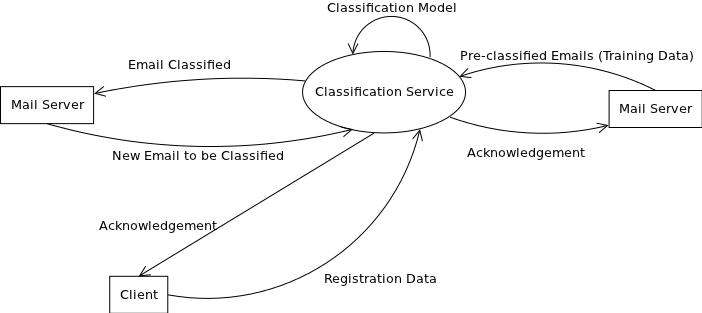
\includegraphics[width=13cm]{context_diagram.png}
  \caption[The Context Diagram illustrates the modules, business processes, ...etc that feed 
or interact with this proposed application.] {The Context Diagram illustrates the modules, business processes, ...etc that feed 
or interact with this proposed application.}
\end{figure}


%==============================================================================
\subsubsection{High Level Workflow}
The workflow required to complete the primary objectives of the proposed 
application is described below. The workflow is business-centered, and 
includes ``decision forks'' for decisions the business user, or application, 
must make to achieve the objective. The workflow omits application faults or exceptions. 
Individual tasks in the workflow are described.

\begin{my_enumerate}
  \item Workflow/Process Map 
	
\begin{figure}[H]
  \centering
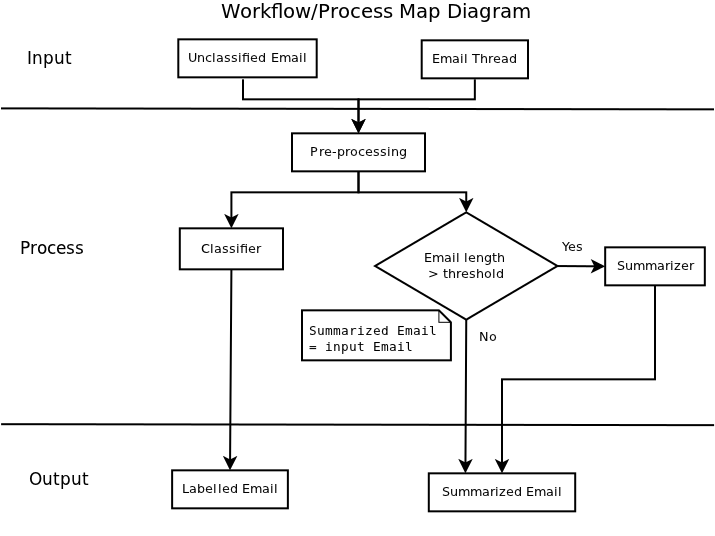
\includegraphics[width=13cm]{workflow_process_map.png}
  \caption[Workflow Process] {Workflow Process}
\end{figure}

  \item Workflow Description
  \begin{my_itemize}
    \item Incoming Emails are preprocessed.
    \item Classification module uses the user model to classify the email into a specific label.
    \item The result is returned by the web service.
  \end{my_itemize}
\end{my_enumerate}

%==============================================================================
\subsubsection{User stories}
Breaking up the system components to user stories with estimated time (in terms
of man-days = 4 hours) to finish the story is very good practice.
\\

\begin{tabular}{|p{3cm}|p{10cm}|}
\hline
\cellcolor[gray]{0.9} Story Id & \#1 \\ \hline
\cellcolor[gray]{0.9} User Story & Authentication \\ \hline
\cellcolor[gray]{0.9} Priority & Low \\ \hline
\cellcolor[gray]{0.9} Description & 
      As a \textbf{User}, I can \textbf{authenticate the application}. \\ \hline
\cellcolor[gray]{0.9} Estimated time & 1 man-day \\ \hline
\cellcolor[gray]{0.9} Notes & 
      Authentication is done with email username and password. \\ \hline
\end{tabular}

\begin{tabular}{|p{3cm}|p{10cm}|}
\hline
\cellcolor[gray]{0.9} Story Id & \#2 \\ \hline
\cellcolor[gray]{0.9} User Story & Deauthentication \\ \hline
\cellcolor[gray]{0.9} Priority & Low \\ \hline
\cellcolor[gray]{0.9} Description & 
	As a \textbf{User}, I can \textbf{deauthenticate the application}. \\ \hline
\cellcolor[gray]{0.9} Estimated time & 1 man-day \\ \hline
\cellcolor[gray]{0.9} Notes & 
	Authentication is done with email username and password. \\ \hline
\end{tabular}

\begin{tabular}{|p{3cm}|p{10cm}|}
\hline
\cellcolor[gray]{0.9} Story Id & \#3 \\ \hline
\cellcolor[gray]{0.9} User Story & Label suggestion \\ \hline
\cellcolor[gray]{0.9} Priority & Medium\\ \hline
\cellcolor[gray]{0.9} Description & 
	As a \textbf{User}, I can \textbf{give feedback for the chosen/suggested labels} to
	\textbf{enhance the classification accuracy}. \\ \hline
\cellcolor[gray]{0.9} Estimated time & 5 man-days\\ \hline
\cellcolor[gray]{0.9} Notes & 
	Build browser extension to support suggestions in gmail. \\ \hline
\end{tabular}

\begin{tabular}{|p{3cm}|p{10cm}|}
\hline
\cellcolor[gray]{0.9} Story Id & \#4 \\ \hline
\cellcolor[gray]{0.9} User Story & Data pre-processing \\ \hline
\cellcolor[gray]{0.9} Priority & High\\ \hline
\cellcolor[gray]{0.9} Description & 
	As a \textbf{System}, I can \textbf{preprocess the dataset} to
	\textbf{make it ready for the classification}. \\ \hline
\cellcolor[gray]{0.9} Estimated time & 4 man-days\\ \hline
\cellcolor[gray]{0.9} Notes & 
	Preprocessing includes stemming, checking email length/language,
	removing stop words and identifying the features. \\ \hline
\end{tabular}

\begin{tabular}{|p{3cm}|p{10cm}|}
\hline
\cellcolor[gray]{0.9} Story Id & \#5 \\ \hline
\cellcolor[gray]{0.9} User Story & Email Classification \\ \hline
\cellcolor[gray]{0.9} Priority & High\\ \hline
\cellcolor[gray]{0.9} Description & 
	As a \textbf{System}, I can \textbf{make online classification to
	an incoming email}. \\ \hline
\cellcolor[gray]{0.9} Estimated time & 20 man-days\\ \hline
\cellcolor[gray]{0.9} Notes & 
	More than one algorithm will be implemented to choose the one with 
	the best accuracy. \\ \hline
\end{tabular}

\begin{tabular}{|p{3cm}|p{10cm}|}
\hline
\cellcolor[gray]{0.9} Story Id & \#6 \\ \hline
\cellcolor[gray]{0.9} User Story & User Classification Model \\ \hline
\cellcolor[gray]{0.9} Priority & High\\ \hline
\cellcolor[gray]{0.9} Description & 
	As a \textbf{System}, I can \textbf{build a user classification 
	model from the training data}. \\ \hline
\cellcolor[gray]{0.9} Estimated time & 5 man-days\\ \hline
\cellcolor[gray]{0.9} Notes & 
	It will start after user authentication, and can be applied 
	from time to time to enhance the user model. \\ \hline
\end{tabular}

\begin{tabular}{|p{3cm}|p{10cm}|}
\hline
\cellcolor[gray]{0.9} Story Id & \#7 \\ \hline
\cellcolor[gray]{0.9} User Story & Classification Accuracy test \\ \hline
\cellcolor[gray]{0.9} Priority & Medium \\ \hline
\cellcolor[gray]{0.9} Description & 
	As an \textbf{Admin}, I can \textbf{test the accuracy of the 
	classification algorithm at runtime}. \\ \hline
\cellcolor[gray]{0.9} Estimated time & 2 man-days\\ \hline
\cellcolor[gray]{0.9} Notes & 
	The admin can view the accuracy of the used classification algorithm. \\ \hline
\end{tabular}

%==============================================================================
\newpage
\subsection{Business Requirements}

This section identifies, enumerates and explores the business requirements that must 
be met by the application. Business requirements include capturing the types of users, 
the basic inputs and outputs, the system's dependencies, and the tasks the system should 
accomplish. It is important to confirm that Task Requirements include all the tasks 
required to meet the business objectives.

%==============================================================================
\subsubsection{Users}
All applications have users and most of them have several users of different types. This 
section identifies, at a high level, the types of users of the system.

\begin{my_enumerate}
  \item Application User: requests emails classification.
  \item Admin: tunes classification algorithms and observes the results.
\end{my_enumerate}

%==============================================================================
\subsubsection{Inputs/Outputs}
This section identifies and describes the inputs to and outputs from the new 
application. In this section, all electronic inputs and outputs 
are captured. Human inputs are omitted from this section.

\begin{my_enumerate}
  \item Inputs:
  \begin{my_itemize}
    \item unclassified Emails;
    \item classified Emails (training data);
  \end{my_itemize}
  \item Outputs:
  \begin{my_itemize}
    \item classified emails;
    \item classification model.
  \end{my_itemize}
\end{my_enumerate}


%==============================================================================
\subsubsection{Dependencies}
Human inputs are also categorized as dependencies.
\begin{my_enumerate}
  \item IMAP service in the email provider.
  \item Registration data.
  \item Number of emails in each user-defined label (affects classification model)
\end{my_enumerate}


%==============================================================================
\subsubsection{Security Requirements}
This section documents, at a high level, the basic security requirements of the 
application. For example, does the system require the user to login?  Should the 
user’s identity be authenticated on just this system, or against a central authority?  
Are there any special or unusual security requirements, like fingerprint scanning?

\begin{my_enumerate}
  \item The system requires every user to login with a unique identity (email).
  \item User Data (email) should be transmitted through a secure connection.
  \item Administrators shouldn’t have access to user data (email).
\end{my_enumerate}



%==============================================================================
\subsubsection{Performance Requirements}
Performance Requirements for the application are defined at a high level below. 
If there are specific requirements for specific features to perform at a quantifiable 
level, they too are listed below. These requirements will be developed in more detail when 
the Requirements Specification is written, in a later phase.

\begin{my_enumerate}
  \item Classification web service should respond within a reasonable time.
  \item Initial training phase should finish within a reasonable time.
  \item The system will achieve high uptime.
\end{my_enumerate}


%==============================================================================
\subsubsection{Data Migration}
Data Migration describes the data that needs to be moved from an older or external 
system to the new system, in order for it to operate at launch. Migration also includes 
data that must be transferred from the new system to another external system. 
Any data migration requirements are listed below.

\begin{my_enumerate}
  \item Users' classified emails for training phase as pre-classified emails are needed to build users' models.
  \item Users' feedback on the results of the classification.
\end{my_enumerate}

%==============================================================================

\section{Software Design Description (SDD)}

%------------------------------------------------------------------------------

\subsection{Purpose}
This section shows how the Smart Email software system will be 
structured to satisfy the requirements identified in the software
requirements specification section. It is a translation of 
requirements into a description of the software structure, software components, 
interfaces, and data necessary for the implementation phase.

\subsection{Scope}
Smart email will provide automated email classification for email clients. 
This section describes how the system will be divided into modules and 
the design details for each module.


\subsection{Decomposition description}
There are three primary stages to the design development which consists of phase 1 
(Classification Web Service Module), phase 2 (Email Monitoring Web Service Module),
and phase 3 (Web Browser Extension).

The classification module can be divided into three layers. The data layer will be 
responsible for retrieving emails from file systems or using IMAP protocol. The 
second layer is the preprocessing and email filtering layer. This layer is 
responsible for filtering emails and extracting classification features from the 
email. The third and last layer will be responsible for classifying emails and 
testing the classifier performance.

The detailed design for each entity is illustrated in the detailed class 
diagram at the end of this section.

\subsubsection{System decomposition}
The system is divided into main modules as follows:
\begin{my_itemize}
  \item classification web service;
  \item email monitoring web service;
  \item web browser extension.
\end{my_itemize}
Each of these modules will be described in details in the upcoming subsections.

\paragraph{Classification Web Service}

Classification web service provides an API for the email classification service.
\begin{my_itemize}
	\item user registeration: A user can register with the service with one or more email accounts. The service trains using the user's email dataset, builds a classification model and stores it in a database.
	
	\item unregisteration: The user can remove himself from the service.

	\item classification request: The user can send a classification request for any email. The system will retrieve the user model, classify the email and send the classification result back to the user.

	\item feedback: In case the system classifies an email to an incorrect folder, the user can send feedback to the system with the correct folder. The system will use this feedback to improve future classification.

\end{my_itemize}

\paragraph{Email Monitoring Web Service} 

Email Monitoring Web Service is a web service implemented in RubyOnRails \cite{ROR} framework which integrates 
with a classification web service for classification of emails. The web service monitors 
users emails and sends every new email to the classification service through a REST API \cite{REST}
which returns a response with the email label, the web service then applies the label to the user’s email.

\begin{itemize}
 \item MVC illustration for the Email Monitoring module
 \begin{figure}[H]
   \centering
   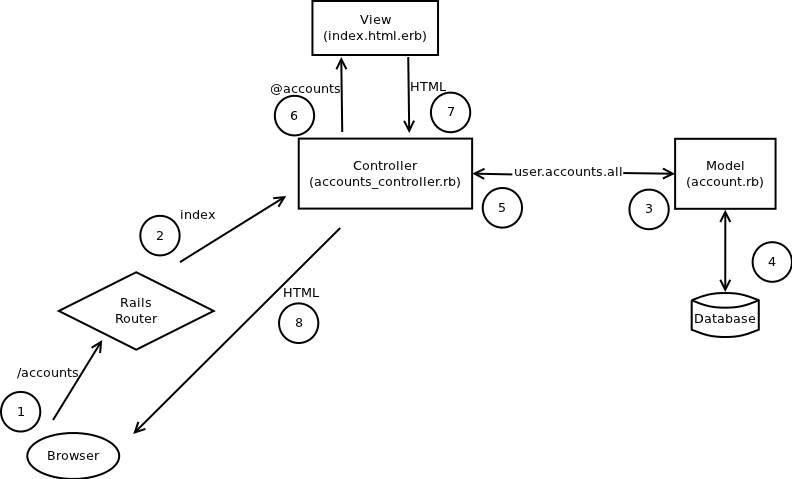
\includegraphics[width=12cm]{account_example.png}
   \caption[Example for MVC in action handling a user request to view his 
   accounts]{Example for MVC in action handling a user request to view his accounts}
 \end{figure}

 \item Features
 \begin{itemize}
    \item Users registration.
    \item Adding more than one email account.
    \item Continuous monitoring of emails accounts for new emails.
 \end{itemize}
 
 \item Future Work
  \begin{itemize}
    \item Providing statistics about the classification process.
    \item Support email providers other than Gmail: Yahoo, Hotmail, ...etc.
    \item Classifying users into active and non-active ones based on their 
    email account activity to decrease the load and increase the performance 
    of the monitoring process.
    \item Improving performance and security.
  \end{itemize}
\end{itemize}

\paragraph{Web Browser Extension}
Web Browser Extension is a client side browser extension that injects a 
``Classify Me'' button when the user open the email which is an additional 
UI component injected into the user's email web interface. 


\begin{itemize}
 \item Features
 \begin{itemize}
    \item Users registration.
    \item Sending a classification requests to the classification web service.
    \item Check the status of the user's training phase at the classification 
    web service.
    \item Sending feedback to the classification web service when the user
    applies labels manually to an email to re-train the model.
 \end{itemize}
 \item Future Work
  \begin{itemize}
    \item Providing statistics about the classification process.
    \item Support other web browsers other than Chrome extension: Firefox, 
    Safari, ...etc.
    \item Improving performance and security.
  \end{itemize}
\end{itemize}

\subsubsection{Data decomposition}
The data layer is responsible for retrieving emails either from the file system or using 
the IMAP protocol. The Enron dataset \cite{ENRON} will be used as the data source for training and 
testing the email classifier.

\begin{my_desc}
  \item[Data access object] this class is used to provide an abstract way to retrieve emails.
  \item[IMAP Data access object] it is responsible for retrieving emails using the IMAP protocol,
  and it inherits the Data access object class.
  \item[File system data access object] it is responsible for retrieving emails from the file
  system, and it inherits the Data access object class.
\end{my_desc}


%==============================================================================
\subsection{Interface description}
The interface description provides everything designers, programmers and 
testers need to know how to correctly use the functions provided by the system 
entities. This description includes the details of external and internal 
interfaces not provided in the software requirements specification.

\subsubsection{Module interface}
\paragraph{Classification Web Service API}
%\begin{itemize}
    \begin{itemize} %TODO: edit this to the new REST API
      \item register(username,password) adds user to database and starts training phase
      \item remove(username,password) removes user information from database.
      \item status(username) returns current status of training phase.
      \item classify(emailContent) returns the best category for this email.
      \item classify(email\_imap\_id) returns the best category for this email.
      \item feedback(email\_content,correct\_label) retrains the model using the new instance.
    \end{itemize}
%\end{itemize}

%-------
\newpage
\paragraph{Email Monitoring Web Service API}
\begin{itemize}
	\item API for user registration
	\begin{itemize}
		\item Basic URL: http://smart-email.herokuapp.com/
		\item Endpoint: /users
		\item Request type: POST
		\item Parameters: username, password
		\item Response: Success/Error on creating the new user
	\end{itemize}

	\item API for email account registration
	\begin{itemize}
		\item Basic URL: http://smart-email.herokuapp.com/
		\item Endpoint: /accounts
		\item Request type: POST
		\item Parameters: username, password
		\item Response: Success/Error on creating the new user
	\end{itemize}
\end{itemize}

%==============================================================================
\newpage
\subsubsection{Detailed design}
\paragraph{Classification module detailed design}
.\\
\begin{figure}[H]
  \centering
  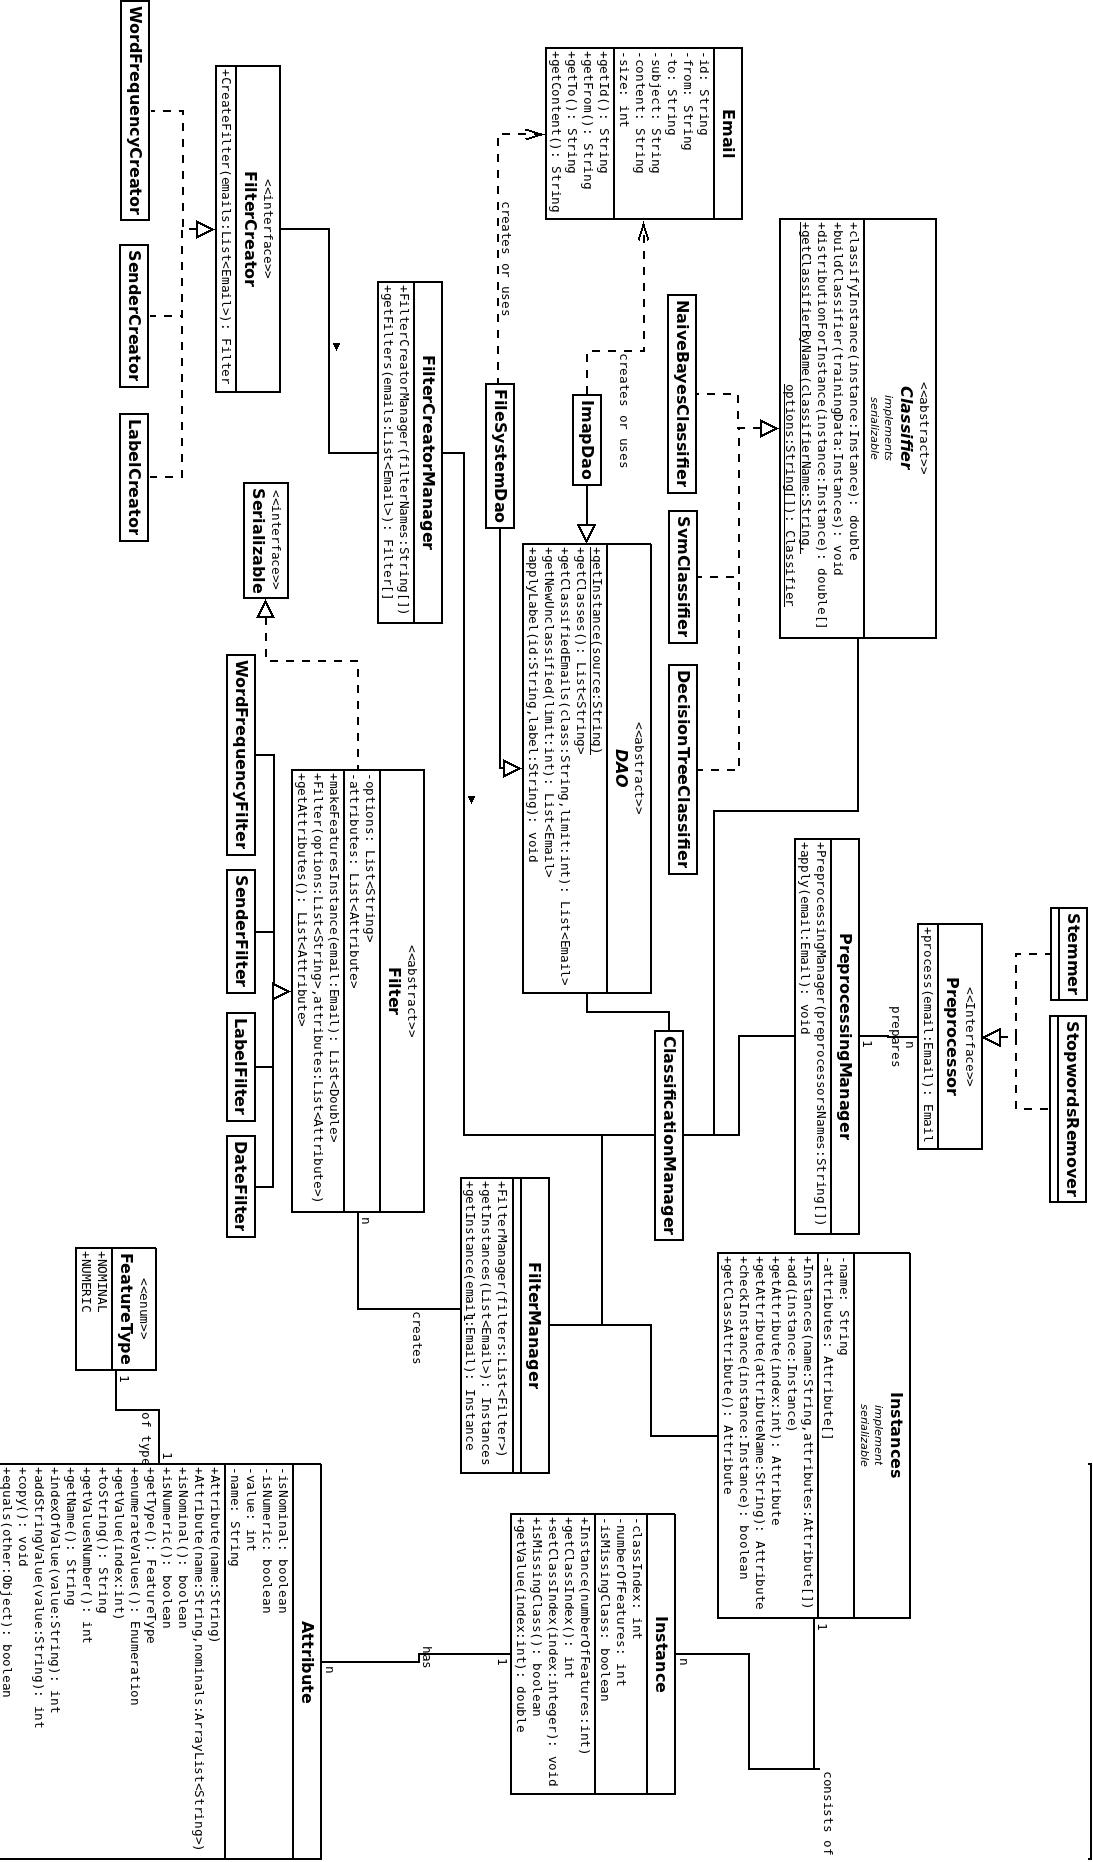
\includegraphics[width=12cm]{design.jpeg}
  \caption[Detailed Design] {Detailed Design}
\end{figure}



\paragraph{Email Monitoring Web service module detailed design}
.\\
\begin{figure}[H]
  \centering
  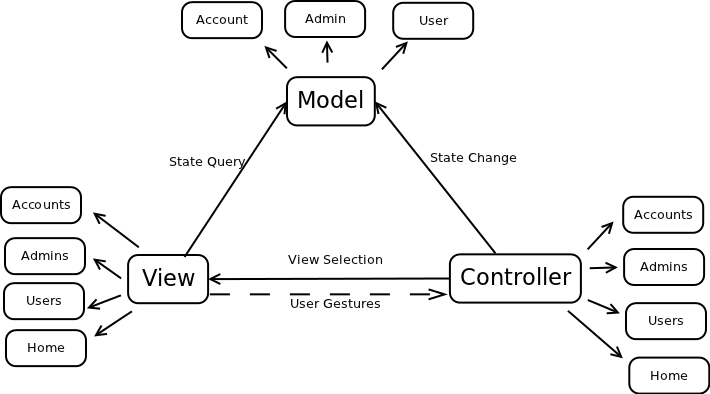
\includegraphics[width=15cm]{mvc2.png}
  \caption[Smart Email MVC Design]{Smart Email MVC Design}
\end{figure}


\section{Conclusion}
In this chapter, the software requirements specification and software design
description were discussed. While in the next chapter, Environment and 
Development tools will be discussed.

% Chapter 5

\chapter{Development Process, Environment and Tools} % Main chapter title

\label{Chapter5} % For referencing the chapter elsewhere, use \ref{Chapter5} 

\lhead{Chapter 5. \emph{Development Process, Environment and Tools}} % This is for the header on each page - perhaps a shortened title

\section{Introduction}
In Chapter 4, Smart Email architecture and design was discussed. In This Chapter, 
the adopted process is examined in details; the stages of work, the tools used 
and the work environment.

The environments needed to be set up are discussed in section 5.2. In section 5.3, 
the software engineering model followed throughout the project will be explained. 
In section 5.4, the development process will be described in details. In section 5.5, 
all the tools used will be explained. In section 5.6 the hardware and software 
environments will be described in details.
%----------------------------------------------------------------------------------------
\section{Setting Up The Environment}
The needed Environments for the project to run
\begin{itemize}
\item Any operating system that is compatible with java Runtime Environment.
\item Java runtime environment.
\item Tomcat 6 server.
\item MySql database.
\end{itemize}

%--------------------------------------------------------
\section{Software Engineering Process Followed}
Since the project included many different processes and stages. A long time is spent and multiple team members were working on it. It was critical to follow a standard methodological software engineering model to keep the work organized and fully utilize the effort.


Software Process Improvement (SPI) for Small Medium Enterprises (SMEs)
model is a model developed by software Engineering Competence Center
whose goal is to help small and medium enterprise to raise the quality of
their products by using modern software development processes and practices. It consists of several processes: the management, development, peer-review, quality assurance and configuration management processes. Since
the SPI model targets mainly enterprise and business, it was required to
slightly modify it to fit scientific natural of the project. Three of these processes were followed in the work which are the development, peer review and
configuration management processes.

\begin{itemize}
\item Development Process: the development processes contained several
phases so it will be discusses in next section 5.4 .
\item Peer review Process: peer review allows to detect the errors early and
almost all team members share their thoughts in the same point and
look at it from many points of view. Throughout the project, all work
was reviewed among the team members.
\item Configuration Management Process: concerned with controlling and
reporting changes during the project's lifetime. During the implementation phase, the source code was edited frequently and by multiple
team members. So configuration management was applied by using
source control system.
\end{itemize}

%--------------------------------------------------------
\section{Development Process}

The development process adopted through the project included the following
phases: requirements specification, planning.

\subsection{Requirements Specification}
Extracting the requirements is considered one of the most important phases
in any software development. The main requirement was a classification web service with a REST api \cite{REST}.
\subsection{Planning}
To achieve the main requirement, several sub-requirements were planned.
First, it was important to compare between classification algorithms and choose a subset of them to use,
then choosing the best Email feature combination to give the highest accuracy,
then choosing the api syntax for the classification web service.
Finally, building a web monitoring web service and a browser extension to demonstrate the capabilities of the classification web service.
\subsection{Analysis}
As stated in the planning phase, Classification algorithms were analyzed and several Email features were compared ,
the results of this comparisons are discussed in chapter 6.
Enron dataset was used to do the analysis. The largest 7 users were chosen to do the analysis \cite{RON04}.

\subsection{Design}
Since several algorithms and features combinations are analyzed and compared , a flexible design that enables changing
the classification algorithm or the classification feature were needed.
Design is described in details in the previous chapter.

\subsection{Implementation}
The implementation phase was the most time demanding phase in the
project.
The implementation phase was divided into 3 parts.
First implementing the classification web service using JavaEE and REST api \cite{REST},
then implementing the email monitoring web service using ruby on rails \cite{ROR}
and finally the browser extension using google chrome browser extension api \cite{CHROME}.
\subsection{Integration}
After implementing the classification web service,
it was required to integrate the email monitoring web service and the browser extension with
the classification web service and make sure they can communicate with the classification web
service using the REST api.

\subsection{Testing}
Several levels and types of testing were applied throughout the project.
\begin{itemize}
\item Unit testing was applied on several standalone modules.
\item Integration testing was applied to the classification service as a whole.
\end{itemize}
\subsection{Deployment}
The classification web service was configured so that it can be deployed on any web server that supports javaEE.
The email monitoring web service was deployed to heroku \cite{HEROKU}.
The chrome browser extension can be deployed to chrome extension web store.

%--------------------------------------------------------
\section{Tools Used}

\subsection{Programming Languages Used}
\begin{itemize}
\item Java Enterprise Edition version 6 was used as the main language in the classification web service.
\item Ruby on rails \cite{ROR} was used for developing the email monitoring web service.
\item Javascript was used for developing the browser extension.
\end{itemize}

\subsection{Integrated Development Environments (IDEs)}
Eclipse IDE was used for the classification web server.
Vim text editor was used for developing the browser extension and the email monitoring web service.
\subsection{Web Servers}
The following web servers were used
\begin{itemize}
\item Tomcat 6 is used as a java web server for the classification web server.
\item Rails web server as a server for the email monitoring web server.
\end{itemize}

\subsection{Source Control}
git source control system \cite{GIT} was chosen to allow versioning and provide the ability to rollback to any version of the project.
%--------------------------------------------------------
\section{Hardware And Software Environment}

%--------------------------------------------------------
\section{Conclusion}
In this chapter, the development process, used tools and project environment were discussed in depth. In the next chapter, an analysis for the classification procedure is provided.

% Chapter 6

\chapter{Implementation, Results and Discussion} % Main chapter title

\label{Chapter6} % For referencing the chapter elsewhere, use \ref{Chapter6} 

\lhead{Chapter 6. \emph{Implantation, Results and Discussion}} % This is for the header on each page - perhaps a shortened title

%----------------------------------------------------------------------------------------

\section{Introduction}
In Chapter \ref{Chapter5}, the adopted development process, the tools used and the work environment were examined in details.

In this chapter, implementation details and results are discussed. In section
\ref{sec:6_imp_details}, implementation details of the classification web service,
email monitoring web service, and Chrome extension are discussed. While in section
\ref{sec:6_results_discussion}, experiments of different classification procedures,
dataset splits, feature selection, and analysis of the obtaind results are presented. 
And the chapter is concluded in section \ref{sec:conclusion_6}.

%==============================
\section{Implementation Details}
\label{sec:6_imp_details}
%==============================

\subsection{Classification Web Service implementation details}
This section will discuss the implementation details of the classification web service.


    \subsubsection{Training Phase}
    Once the user registers in the classification web service, Smart Email will start downloading pre-classified emails from
    user email provider using IMAP protocol.

    Smart Email design described in the previous chapter is flexible and enables using different data sources,a file data source was used
    to read Enron \cite{ENRON} dataset from file system.

    Other protocols can be implemented like POP3.

    \subsubsection{Preprocessing phase}
    Smart Email uses several preprocessors on incoming emails. The following are the currently implemented preprocessors,
    the design of the Smart Email allows the addition of other preprocessors without modification to the existing code.
        \begin{description}
        \item[Stemming] Porter stemmer \cite{STEMMER} is used to stem words of email.
        \item[Stop words removal] is used to remove stop words like ("the","them",.. etc).
        \item[Lowercasing] is used to convert all words in subject and body to lowercase.
        \item[Number Normalization] is used to convert all numbers to a specific tag.
        \item[URL Normalization] is used to convert all urls into specific tags.
        \item[HTML tags remover] is used to remove html tags from emails if they exist.
        \end{description}

    \subsubsection{Classification phase}
    When a new Incoming Email is sent to the classification web service,
    the email is preprocessed as described above and features (described in details in Chapter \ref{Chapter3}
    are extracted to build the input tuple.

    The input tuple is then given to WEKA \cite{WEKA} (Naive Bayes or SVM) classifier to 
    perform the classification. The result of the classification is then returned.

\subsection{Email monitoring web service implementation details}
    Users register in the email monitoring web service by providing user name and password,
    then the user can add one or more email accounts to be monitored.
    A Job runs in the background opening IMAP-IDLE connection for every user's email account.
    This job sends every new incoming email to the classification web service and
    applies the returned label to user's email.

    This web service was built using Ruby on Rails \cite{ROR} framework, MySQL database was used
    in development environment while postgresql was used in production.


\subsection{Chrome Browser Extension implementation details}
    Chrome Extension is a client side extension for the Google chrome browser \cite{CHROME}.
    The extension injects a javascript file in the gmail web interface. The extension also manipulates
    gmail web interface HTML page by injecting a button entitled ``Classify Me''
    that appears when the user selects any email to view.

    The button is injected by adding a new DOM element to the html page.The extension must waits till
    the page completely loads to do the injection.

    When the user clicks the ``Classify Me'' button the extension retrieves the raw email and
    builds a message using the raw email,an ajax call with the message is made to the 
    classification web service.

    The extension also detects when the user tries to manually classify an email, The extension builds
    a feedback message with the email and the correct label, then sends it to the classification 
    web service.

    To detect events like manual classification, the extension must intercepts ajax requests made by
    gmail and examines the request body.

    The Extension uses the Gmailr library \cite{GMAILR} to detect various events. The library was modified 
    to be able to detect "apply new label" event.

%--------------------------------------------------------------------------------------
\section{Results and Discussion}
\label{sec:6_results_discussion}
\subsection{Experimental Setup}

\subsubsection{Enron Dataset \cite{ENRON}}
Enron dataset is the most popular email corpus for research. It was released 
during the legal investigation into the Enron corporation.
It is an invaluable dataset since it contains uncensored messages from a 
corporate environment. The dataset consists of employee's email folders, 
so it is also an accurate depiction of how users use folders. The majority 
of email directories in the dataset are small, so seven users with the largest 
email directories are chosen for the experiments. Those seven users are chosen 
in many related papers (e.g. Huang, Bekkerman and McCallum, 2004\cite{RON04}).

Statistics on the seven users are shown in table \ref{enronStatsTable}:

\begin{center}
	\centering
	\begin{table}[H]
		\begin{tabular}{ |  >{\centering} l |  >{\centering} p{1.75cm} |  >{\centering} p{1.75cm} |  >{\centering}p{1.75cm} |  >{\centering} p{1.75cm} |  >{\centering} p{1.75cm} | p{1.75cm} <{\centering} | }
		\hline

		User & Number \newline of \newline folders & Number \newline of \newline messages & Size of \newline smallest \newline folder \newline (messages) & Size of \newline largest \newline folder \newline (messages) & Size of \newline smallest \newline message \newline (words) & Size of \newline largest \newline message \newline (words) \\ \hline \hline

		Beck-s & 101 & 1971 & 3 & 166 & 45 & 2620 \\ \hline
		Farmer-d & 25 & 3672 & 5 & 1192 & 43 & 3507 \\ \hline
		Kamniski-v & 41 & 4477 & 3 & 547 & 44 & 7885 \\ \hline
		Kitchen-l & 47 & 4015 & 5 & 715 & 47 & 46296 \\ \hline
		Lokay\_m & 11 & 2489 & 6 & 1159 & 45 & 4456 \\ \hline
		Sanders\_r & 30 & 1188 & 4 & 420 & 55 & 19331 \\ \hline
		Williams-w3 & 18 & 2769 & 3 & 1398 & 49 & 2287 \\ \hline
		\hline

		\end{tabular}
	\caption{Statistics on Enron datasets after removing non-topical and small folders.}
	\label{enronStatsTable}
	\end{table}
\end{center}



\subsubsection{Experiments}
Two types of experiments are reported:

\begin{itemize}
  \item learning curves (Timeline): A learning curve is done by calculating the 
  accuracy of each training/test split and plotting the classification accuracy 
  curve over the number of training messages in the splits;

  \item feature comparison: Different combinations of possible classification 
  features are selected and the accuracy of each combination is plotted. 
  Each combination is run using both Naive Bayes and SVM algorithms.
  \end{itemize}

\subsubsection{Training/test Set Splits}
In practice, the dataset grows over time. So, a natural way of splitting the 
dataset would be based on time: train on earlier emails and test on later 
ones. A similar approach is employed in (Klimt and Yang, 2004)\cite{KY04}. 
The incremental time-based split is done by sorting the emails according to 
their time stamp, then the classifier is trained on the first N messages and 
tested against the following N messages, then it is trained on the first 2N 
messages and tested against the following N messages ...etc. until we cover 
the whole dataset. N was chosen to be 100 which is similar to experiments 
conducted in (Bekkerman, McCallum and Huang 2004)\cite{RON04}.

\subsection{Results}

\subsubsection{Learning Curves}
Results of the seven Enron users are presented below as the accuracy over 
the timeline for each user.

\begin{figure}[H]
    \begin{center}
    \subfigure[beck-s]{
        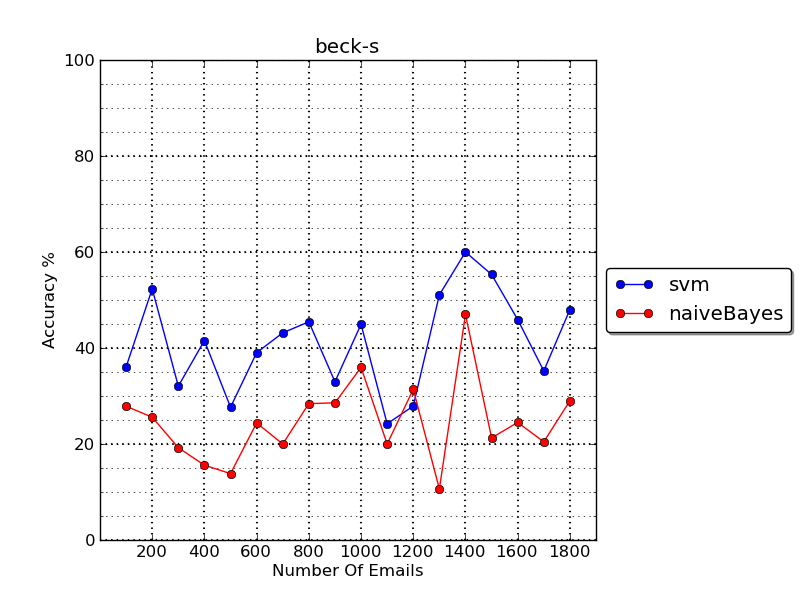
\includegraphics[scale=0.3]{beck-s.png}
    }
    \subfigure[farmer-d]{
        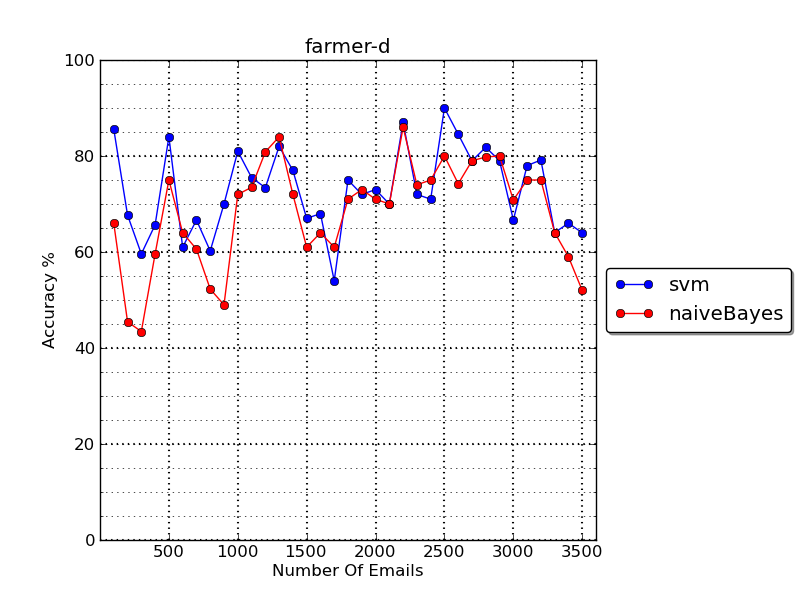
\includegraphics[scale=0.3]{farmer-d.png}
    }
    \subfigure[kamniski-v]{
        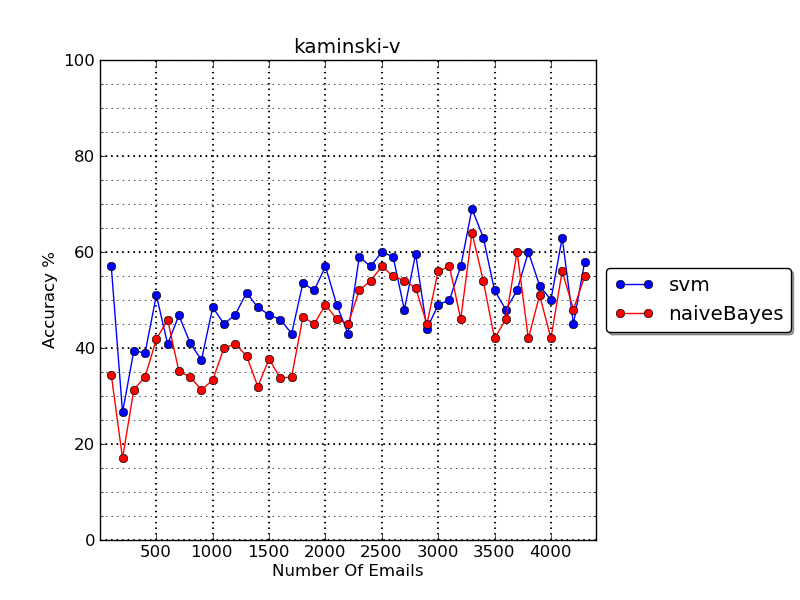
\includegraphics[scale=0.3]{kaminski-v.png}
    }
    \subfigure[kitchen-l]{
        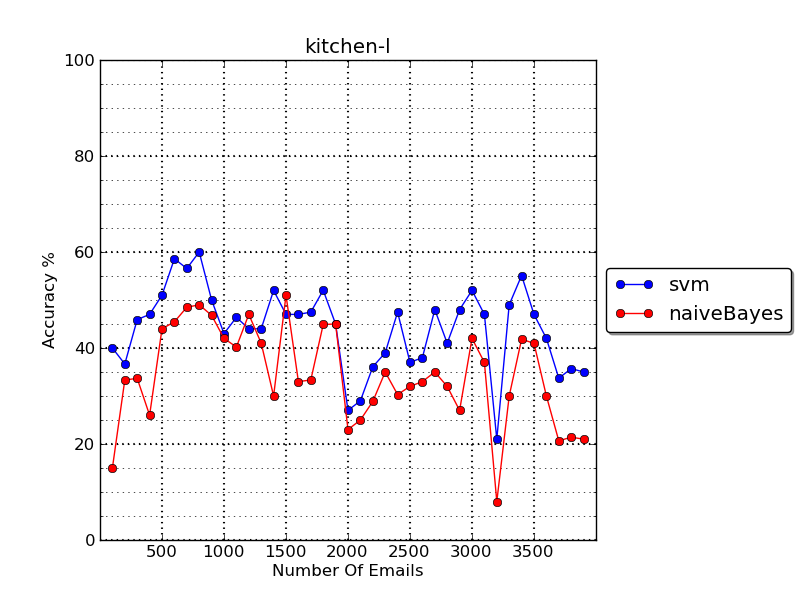
\includegraphics[scale=0.3]{kitchen-l.png}
    }
    \subfigure[lokay\_m]{
        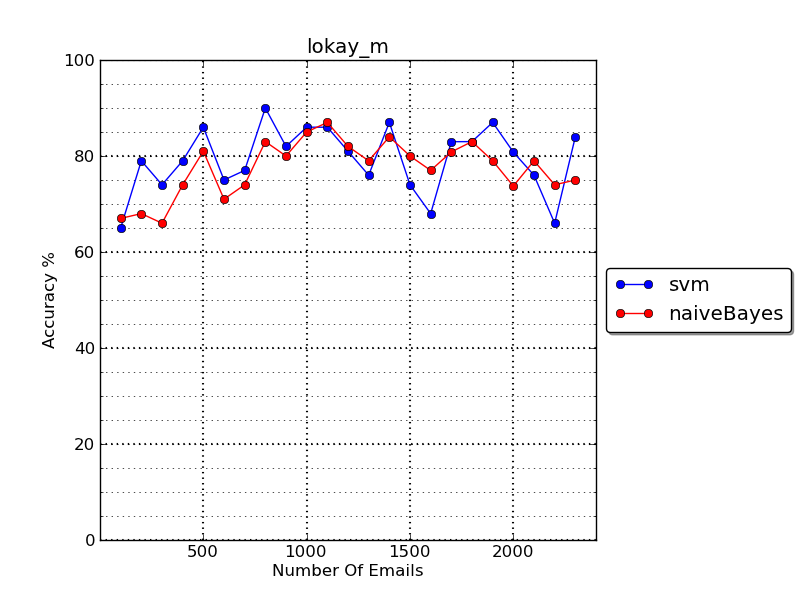
\includegraphics[scale=0.3]{lokay_m.png}
    }
    \subfigure[sanders\_r]{
        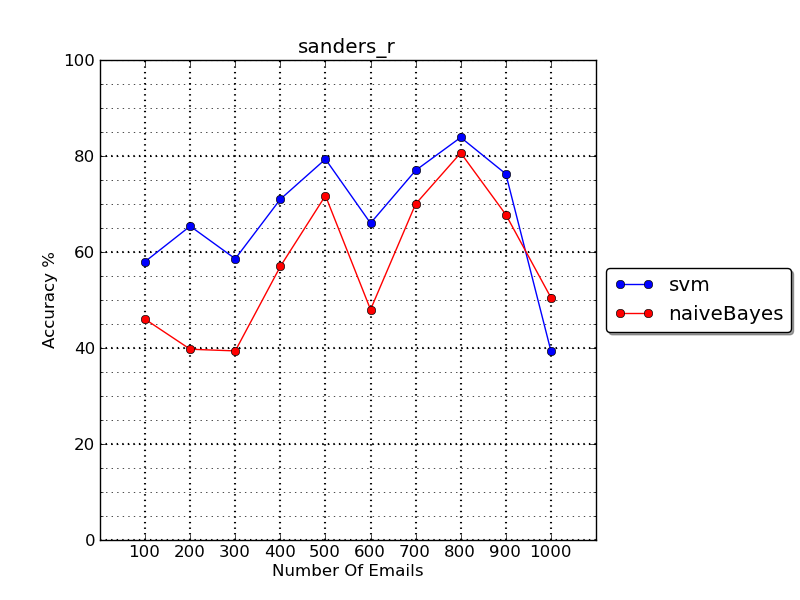
\includegraphics[scale=0.3]{sanders_r.png}
    }
    \subfigure[williams-w3]{
        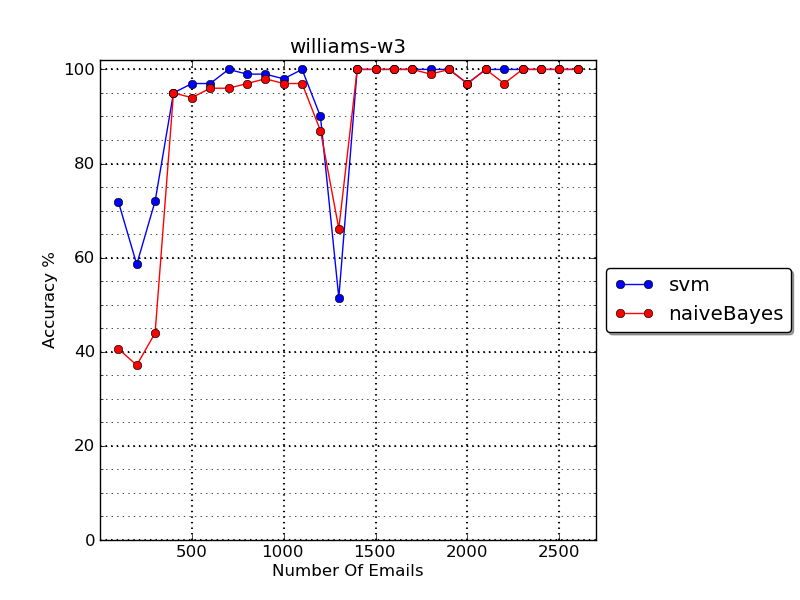
\includegraphics[scale=0.3]{williams-w3.png}
    }
    \end{center}
    \caption{Timeline results (learning curvers)}
\end{figure}

The following table is the accuracies averaged over all training/test splits 
for all users. It has two columns representing the two different classification 
algorithms: Naive Bayes and SVM.

\begin{table} [!htbp]
	\begin{center}

	    \begin{tabular}{ | l | l | l |}
	    \hline
	    User {\textbackslash}  Classifier & Naive Bayes & SVM \\ \hline
	    Beck-s & 24.65\% & 41.27\% \\ \hline
	    Farmer-d & 68.36\% & 72.87\% \\ \hline
	    Kamniski-v & 44.53\% & 50.36\% \\ \hline
	    Kitchen-l & 34.44\% & 44.15\% \\ \hline
	    Lokay\_m & 77.50\% & 79.34\% \\ \hline
	    Sanders\_r & 57.08\% & 67.49\% \\ \hline
	    Williams-w3 & 89.92\% & 93.30\% \\
	    \hline
	    \end{tabular}
	\caption{Average accuracy over all training/test splits}
	\end{center}
\end{table}

\subsubsection{Feature Comparison}
Different combinations of the features affect the accuracy of classifiers. 
It is not necessarily that adding a feature will improve accuracy. So, it 
was important to test different features combinations to select the best 
combination. The results of six different combinations are reported below 
for each user. Each combination is tested under both Naive Bayes and SVM 
classification algorithms.

\begin{figure}[H]
    \begin{center}
    \subfigure[beck-s]{
        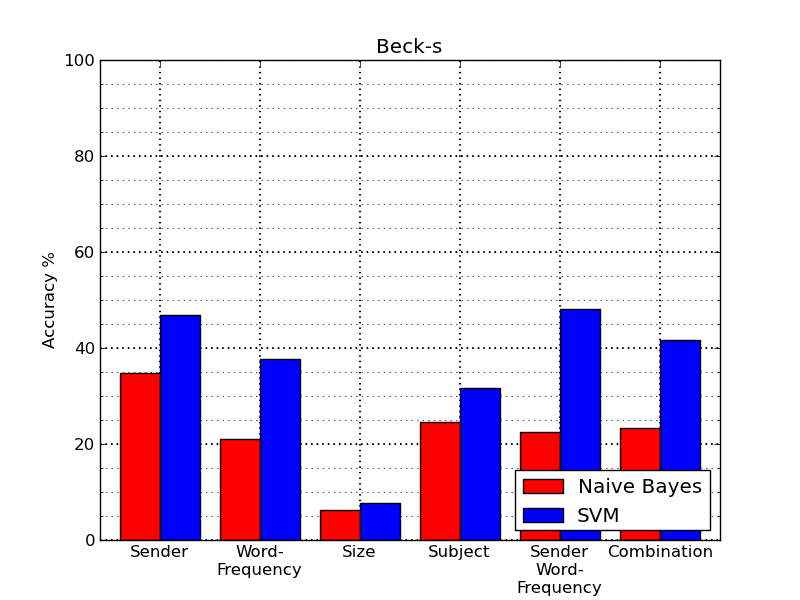
\includegraphics[scale=0.3]{F_Beck-s.png}
    }
    \subfigure[farmer-d]{
        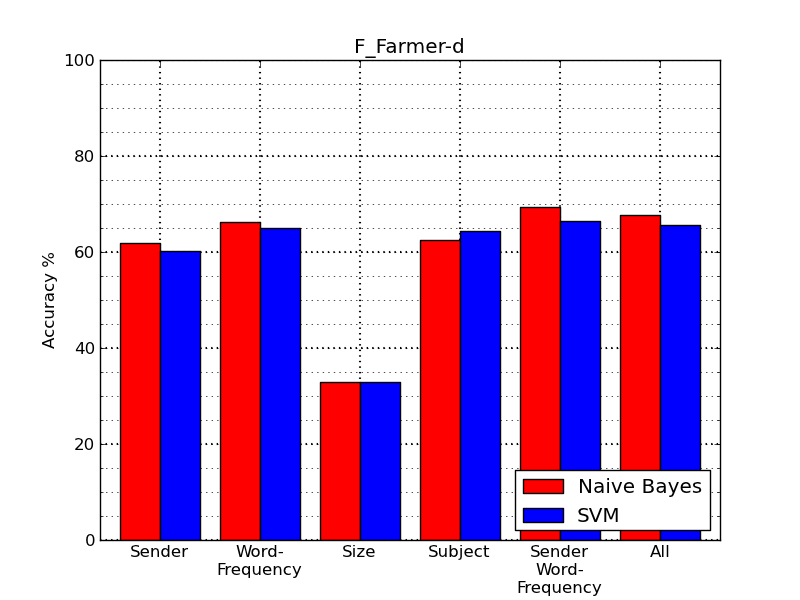
\includegraphics[scale=0.3]{F_Farmer-d.png}
    }
    \subfigure[kamniski-v]{
        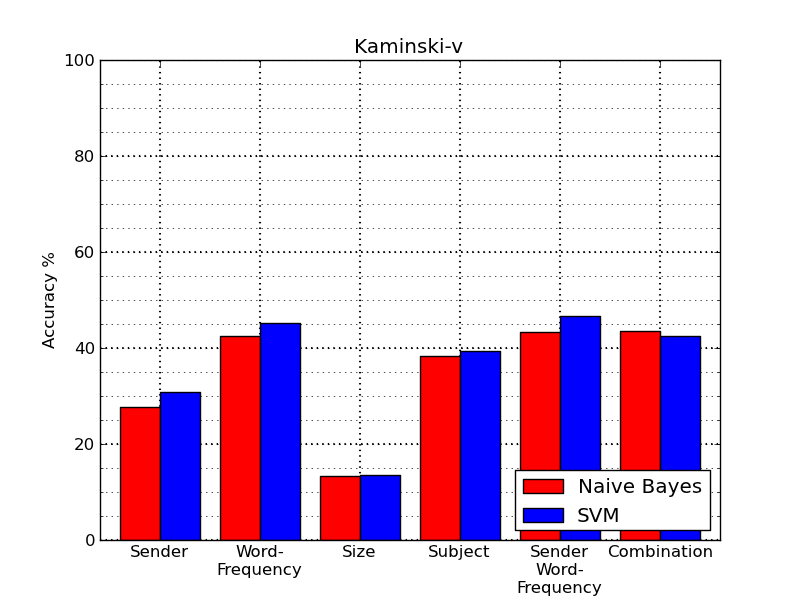
\includegraphics[scale=0.3]{F_Kaminski-v.png}
    }
    \subfigure[kitchen-l]{
        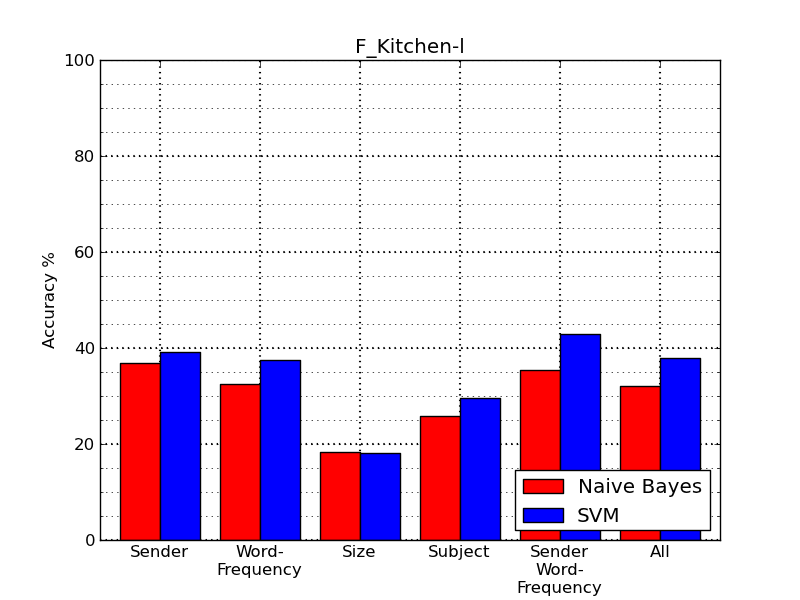
\includegraphics[scale=0.3]{F_Kitchen-l.png}
    }
    \subfigure[lokay\_m]{
        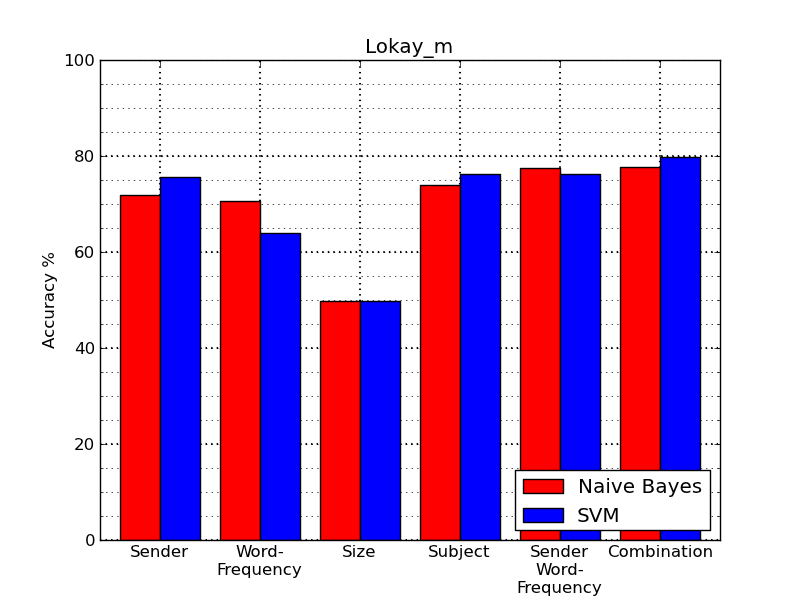
\includegraphics[scale=0.3]{F_Lokay_m.png}
    }
    \subfigure[sanders\_r]{
        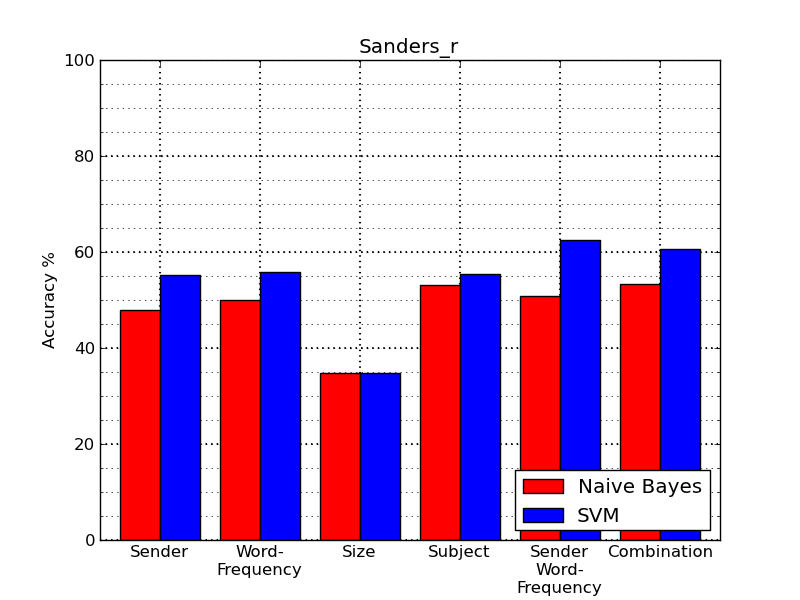
\includegraphics[scale=0.3]{F_Sanders_r.png}
    }
    \subfigure[williams-w3]{
        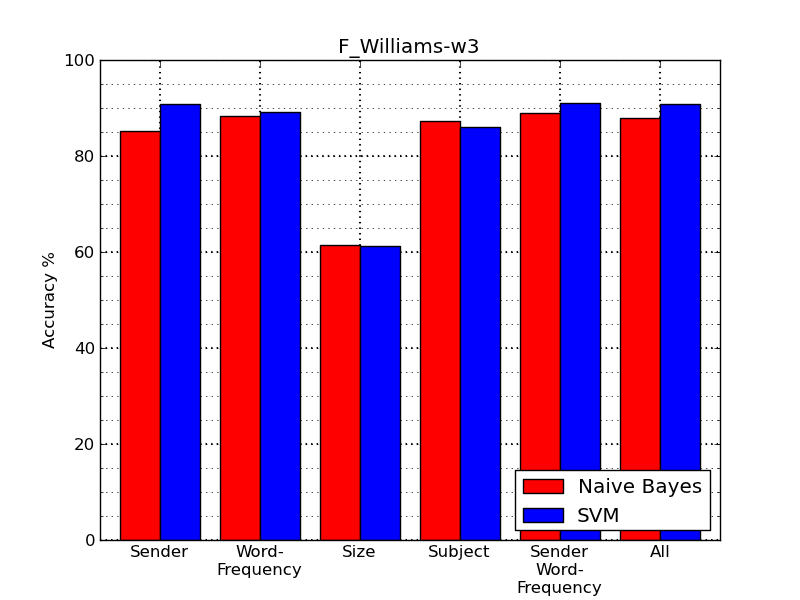
\includegraphics[scale=0.3]{F_Williams-w3.png}
    }
    \end{center}
    \caption{Results of different features combinations}
\end{figure}

%-----------------------------------------------------------------
\subsection{Discussion}
Learning curves (figure 6.1) show that SVM outperforms Naive Bayes in most of 
the cases. This is the expected behaviour. It is widely believed that Naive Bayes 
is not the best algorithm for text categorization (Dumais et al., 1998)\cite{DHS98}.
However, the results obtained doesn't reveal significance superiority of SVM over 
Naive Bayes. In fact, in some cases Naive Bayes was better than SVM (e.g Farmer-d 
feature selection figure). This is probably due to features selection and how 
the classifier weights each feature.


Experimental results obtained support the following observations
\begin{itemize}
  \item Accuracies are higher when the dataset has one or two dominant folders. 
  As it can be seen from Table \ref{enronStatsTable} the size of the largest folder 
  is nearly one half size of the entire dataset (e.g., users lokay\_m and williams-w3).

  \item Newly created folders negatively affect the classification accuracy. If a new 
  folder is created, the classifier trains on few emails from this folder which may 
  not be enough to build a good classification model. (e.g see the drops in figures 
  (6.1-f) and (6.1-g))

  \item The dataset of user williams-w3 (figures (6.1-g) and (6.2-g)) is a degenerative 
  case. It has two large folders (``bill williams iii'' and ``schedule crawler'' which 
  contain most of the messages. This explains the high accuracy for this dataset regardless 
  of features used.

  \item Classification using the sender feature alone yields good results (figure 6.2).

  \item Using both the sender feature and the bag of words (word frequency) feature 
  achieves best results in most of the cases. Adding more features doesn't necessarily 
  improve the accuracy.

  %TODO add more points (about feature comparison)
\end{itemize}

\section{Conclusion}
\label{sec:conclusion_6}
In this chapter the implementation details, results and discussion were presented. In section 
\label{sec:6_imp_details} The implementation details of the classification web service, 
email monitoring web service and chrome extension were presented in details.

In section \label{sec:6_results_discussion} the experimental results were presented.
Analysis of the results were discussed. The results reveal the difficulty of email 
classification. Improving the accuracy is listed as a future work.


% Chapter 7

\chapter{Conclusion And Future Work} % Main chapter title

\label{Chapter7} % For referencing the chapter elsewhere, use \ref{Chapter6} 

\lhead{Chapter 7. \emph{Conclusion And Future Work}} % This is for the header on each page - perhaps a shortened title

%----------------------------------------------------------------------------------------


\section{Conclusion}
In chapter 1, the project's main idea was illustrated which
is a web service that provides automatic email categorization into
user-defined folders based on machine learning and data mining
classification techniques.

A classification web service was built with REST API \cite{REST} that receives
classification requests with the required email to be classified and returns
the most suitable category for this mail.

An Email monitoring web service was built as a client for the classification
web service mentioned above. Users can register in this web servers to have
their email accounts continuously monitored and their incoming emails automatically
classified to the best category.

A Google Chrome Browser \cite{CHROME} Extension was built as another example of a
classification web service client. The Extension provides google chrome users
with a graphical user interface that is integrated with gmail web interface.
Using this extension , Users can send email classification requests on demand.
The extension also detects manual classification done by the user to be sent
for the classification web service as a feedback on the classifier to learn
from the users classification pattern.
%================================================
\section{Future Work}
In the previous section, the implemented features were stated. In this section
the new features that could be added to Smart Email will be introduced.

\subsection{Future work related to classification web service:}
\begin{itemize}
    \item Security issues : Emails privacy and security are considered very
    important issues, so an additional security to communication between clients and
    web service need to supported;
    \item Multi-Label email classification : Currently the classification web
    service assigns each email only one label. Support for multi-label
    classification can be added.
\end{itemize}

\subsection{Future work related to other Smart Email components:}
\begin{itemize}
    \item To complete the vision of smart email ,
        summarization of email threads can be supported.
    \item Supporting other browsers like (Gmail, Yahoo and Hotmail);
    \item Building a Mobile client for the classification web service.
\end{itemize}




%----------------------------------------------------------------------------------------
%	THESIS CONTENT - APPENDICES
%----------------------------------------------------------------------------------------

\addtocontents{toc}{\vspace{2em}} % Add a gap in the Contents, for aesthetics

\appendix % Cue to tell LaTeX that the following 'chapters' are Appendices

% Include the appendices of the thesis as separate files from the Appendices folder
% Uncomment the lines as you write the Appendices

% Appendix A

\chapter{Summary for Email Classification Research Papers} % Main appendix title

\label{AppendixA} % For referencing this appendix elsewhere, use \ref{AppendixA}

\lhead{Appendix A. \emph{Email Classification Papers Summary}} % This is for the header on each page - perhaps a shortened title

\subsubsection{Automatic Categorization of Email into Folders \cite{RON04}}

\paragraph{Year} 2004
\paragraph{Citations} 112
\paragraph{Introduction}
\begin{my_itemize}
  \item Users get alot of emails this days, not just spam but a large number of 
    legitmate emails also that they need to process in a short time.
  \item The paper shows the results of an extensive benchmark on two large corpora 
    (Enron, SRI) of 4 classification algorithms.
  \item The paper shows an enhancement to the exponential gradient method (winnow).
\end{my_itemize}

\paragraph{Related Work}
\begin{my_itemize}
  \item Clark and Niblet 1989: proposed a rule inductive algorithm CN2 and 
    showed that it can outperform KNN.
  \item Cohen 1996: proposed the RIPPER classifier and showed that it 
	can outperfrom an TF-IDF classifier.
  \item Provost 1999: showed that Na\"{\i}ve Bayes can outperform RIPPER.
  \item Remmie 2000: achieved a very high accuracy by classifying mails to
	3 predefined folders.
  \item Kiritchenko and Malwin 2001: showed that SVM can outperfom Na\"{\i}ve Bayes.
\end{my_itemize}


\paragraph{Algorithms Benchmarked}
\begin{my_itemize}
  \item Maximum Entropy.
  \item Na\"{\i}ve Bayes.
  \item SVM.
  \item Winnow (enhanced version).
\end{my_itemize}

\paragraph{Challenges in mail classification}
\begin{my_itemize}
  \item Email users often create folders and let it fall out of use 
	(small number of training data per folder).
  \item Folders don't necessarily correspond to simple semantic topics 
	(unfinished todos, project groups, certain recipient).
  \item Differ drastically from one user to another.
  \item Email arrives in a stream over time which causes more difficulties, 
	for example the topic of main folder can drift over time.
\end{my_itemize}


\paragraph{Dataset pre-processing}
\begin{my_itemize}
    \item Removing non topical folders (Inbox, sent, trash, ...etc).
    \item Removing small folders (folders that has a small number of emails).
\end{my_itemize}

\paragraph{Training/test set splits}
\begin{my_itemize}
    \item The paper shows a new way to split training data into training set 
	  and test set, the new method takes time factor into considerations.
    \item It works as follows:
    \begin{my_itemize}
        \item sorting emails by time;
        \item train the classifier for the first N emails;
        \item test it on the following N emails;
        \item train the classifier for the first 2N emails;
        \item then test it for the following N emails;
        \item and so on.
    \end{my_itemize}
\end{my_itemize}

\paragraph{Features Extraction}
traditional bag of words representation.


\paragraph{Datasets} 
    \begin{my_itemize}
    \item Enron:
    \begin{my_itemize}
	\item http://www.cs.cmu.edu/$\sim$enron/
        \item 150 users with more than 500,000 emails;
        \item applied to the following 7 employees folder only 
	      (the largest 7 folders: beck-s, farmer-d, kaminski-v, 
	      kitchen-l, lokay-m, sanders-r, and williams-w3);
        \item removed the non topical folders like ``all documents'', 
	      ``calendar'', ``contacts'', ``deleted items'', ``discussion threads'', 
	      ``inbox'', ``notes inbox'', ``sent'', ``sent items'', and ``sent mail'';
        \item flatten all the folder hierarchies;
        \item removed folders with less than 3 messages;
        \item removed the X-Folder field from email messages. (The X-Folder 
	      field contains the class label).
    \end{my_itemize}
    \item SRI:
    \begin{my_itemize}
	\item http://www.ai.sri.com/project/CALO
        \item applied to the following 7 folders only: acheyer, bmark, disrael, 
	      mgervasio, mgondek, rperrault, and vchaudri;
        \item removed the non topical folders (inbox, draft, sent, trash);
        \item flatten all the folder hierarchies;
        \item removed folders with less than 3 messages.
    \end{my_itemize}
\end{my_itemize}

\paragraph{Critique}
\begin{my_itemize}
    \item They didn't use Stemming in their preprocessing to the dataset.
    \item Not including precision, recall and f1 score for accuracy measures.
\end{my_itemize}

\paragraph{Conclusion}
\begin{my_itemize}
    \item Na\"{\i}ve Bayes is inferior to other algorithms.
    \item SVM achieved the highest accuracies in most of the tests.
\end{my_itemize}

\paragraph{Future Work}
\begin{my_itemize}
    \item Different sections of each email can be treated differently. 
	  For example, the system could create distinct features for words appearing 
	  in the header, body, signature, attachments, ...etc.
    \item Named entities may be highly relevant features. It would be desirable to 
	  incorporate a named entity extractor (such as MinorThird3, see, e.g., 
	  Cohen and Sarawagi (2004)) into the foldering system.
\end{my_itemize}

%==============================================================================

\subsubsection{Email Classifications For Contact Centers \cite{ANI03}}
\paragraph{Year} 2003
\paragraph{Citations} 14
\paragraph{Main Topic}
\begin{my_itemize}
    \item Proposing an automatic system to classify mail message for contact centers.
    \item Mails are categorized into 2 classes:
    \begin{my_itemize}
        \item single messages: messages that don't require a response;
        \item root messages: messages that require immediate response;
        \item root messages can be sub divided into 3 classes:
        \begin{my_itemize}
            \item root: the start of the communication (contains a problem or a question);
            \item inner: communication on a certain problem;
            \item leaf: marks the end of this interaction (eg. the problem was solved).
        \end{my_itemize}
    \end{my_itemize}
\end{my_itemize}

\paragraph{Tools used}
\begin{my_itemize}
    \item Rainbow: an implementation for Na\"{\i}ve Bayes algorithm.
    \item SVMlight: an implementation for SVM algorithm.
    \item WordNet: used for parts of speach taging.
    \item Ltchunk: used to identify noun phrases and count number of sentences in email.
\end{my_itemize}

\paragraph{Dataset}
\begin{my_itemize}
    \item Pine-info discussion list web archive
    \begin{my_itemize}
        \item http://www.washington.edu/pine/pine-info.
    \end{my_itemize}
\end{my_itemize}

\paragraph{Pre-processing}
\begin{my_itemize}
    \item Removing reply blocks (blocks from previous emails in the current mail).
    \item Removing signature blocks.
\end{my_itemize}

\paragraph{Features (for SVM algorithm)}
\begin{my_itemize}
    \item Non-infected words
    \begin{my_itemize}
        \item nouns, verbs, adjective, adverb;
        \item using WordNet;
    \end{my_itemize}
    \item Noun phrases
    \begin{my_itemize}
        \item using Ltchunk;
    \end{my_itemize}
    \item Verb phrases.
    \item Punctuation letters count.
    \item Length of email (number of sentences)
    \begin{my_itemize}
        \item using Ltchunk.
    \end{my_itemize}
    \item Dictionary
    \begin{my_itemize}
        \item 2 dictionaries were made one for the most common words in single 
	      messages and the other for the most common words in root message.
    \end{my_itemize}
\end{my_itemize}

\paragraph{Conclusion}
\begin{my_itemize}
    \item High accuracy was achieved on root vs leaf (92\%) , root vs inner (87\%) and root vs single(79\%).
\end{my_itemize}


%=================================================================================================

\subsubsection{Using GNUsmail to Compare Data Stream Mining Methods for On-line Email \cite{JOSE11}}
\paragraph{Year} 2011

\paragraph{Citations} 0

\paragraph{Main Topic}
\begin{my_itemize}
    \item Introducing GNUsmail, an open source framework used for mail 
	  classification, focusing on online incremental learning.
    \item Proposing new techniques for testing other than holdout and 
	  cross-validation like prequential measure.
\end{my_itemize}

\paragraph{Evaluation methods}
\begin{my_itemize}
    \item Prequential measure.
    \item Sliding and fading windows.
    \item McNemar test.
\end{my_itemize}

\paragraph{Dataset}
\begin{my_itemize}
    \item Enron.
    \item A layer was added to feed the learning algorithm the new emails one 
	  by one, simulating new incoming emails.
\end{my_itemize}

\paragraph{Algorithms}
\begin{my_itemize}
    \item OzaBag over NNge, using DDM for concept drift detection.
    \item NNge.
    \item Hoeffding Trees.
    \item Majority class.
\end{my_itemize}

\paragraph{Tools}
\begin{my_itemize}
    \item GNUsmail: http://code.google.com/p/gnusmail/.
\end{my_itemize}

\paragraph{Result}
\begin{my_itemize}
  \item Improved GNUsmail by incorporating new different methods to evaluate 
	data stream mining algorithms in the domain of email classification.
\end{my_itemize}

\paragraph{Future Work}
\begin{my_itemize}
  \item Current online learning algorithm implementations have an important 
	limitation that affects the learning process: learning attributes have 
	to be fixed before beginning the induction of the algorithm. They need 
	to know all the attributes, values and classes before the learning itself, 
	since it is not possible to start using a new attribute in the middle of the 
	lifetime of a learning model. Future methods should support online addition of
	new features.
\end{my_itemize}

%=================================================================================================
\subsubsection{E-Classifier: A Bi-Lingual Email Classification System \cite{NOUF08}}
\paragraph{Year} 2008
\paragraph{Citations} 0

\paragraph{Problem}
\begin{my_itemize}
    \item Classifying Arabic and English emails.
    \item Implementing an outlook add-in ``e-classifier''.
\end{my_itemize}

\paragraph{Related Work}
\begin{my_itemize}
    \item English Email Classifiers
    \begin{my_itemize}
        \item PopFile
        \begin{my_itemize}
            \item http://popfile.sourceforge.net.
            \item Uses Na\"{\i}ve Bayes algorithm only.
        \end{my_itemize}
        \item SpamBayes
        \begin{my_itemize}
            \item http://spambayes.sourceforge.net
            \item Binary Classifier (Spam or not).
        \end{my_itemize}
    \end{my_itemize}
    \item Arabic Email Classifiers
    \begin{my_itemize}
    \item There are no Email classification work on arabic language, the
	  related work are on arabic documents not emails El-Kourdiet.
    \end{my_itemize}
\end{my_itemize}

\paragraph{Dataset}
\begin{my_itemize}
    \item English: enron dataset.
    \item Arabic
    \begin{my_itemize}
        \item Translated documents that have been converted to emails.
        \item Documents obtained from http://www.comp.leeds.ac.uk/eric/latifa/research.html.
    \end{my_itemize}
\end{my_itemize}

\paragraph{Pre-processing}
\begin{my_itemize}
    \item English
    \begin{my_itemize}
        \item Removing stop words.
        \item Removing punctuation marks.
        \item Converting all the letters to lowercase.
        \item Porter stemmer.
    \end{my_itemize}
    \item Arabic
    \begin{my_itemize}
        \item No root extraction technique was used due to the lack of non commercial product.
    \end{my_itemize}
\end{my_itemize}

\paragraph{Results}
\begin{my_itemize}
    \item 85\% of English emails were classified correctly.
    \item 60\% of Arabic emails were classified correctly.
\end{my_itemize}

\paragraph{Critique}
\begin{my_itemize}
    \item Used only overall accuracy measure which might not good indicator in case of skewed data.
\end{my_itemize}

%=================================================================================================
\subsubsection{An Object Oriented Email Clustering Model Using Weighted 
	      Similarities between Emails Attributes \cite{NARESH10}}
\paragraph{Year} 2010
\paragraph{Citations}6

\paragraph{Description}
\begin{my_itemize}
    \item Proposing a new Object Oriented Email Clustering Model to categorize 
	  mail message into groups.
\end{my_itemize}

\paragraph{Algorithms}
\begin{my_itemize}
    \item K-means clustering algorithms.
    \item Text similarity techniques.
    \begin{my_itemize}
        \item cosine Similarity.
        \item Dice Similarity.
        \item Blue Similarity.
        \item TF-IDF Similairty (Term Frequency - Inverse Domain Frequency).
        \item Jaccard Similairty.
    \end{my_itemize}
\end{my_itemize}

\paragraph{Datasets}
\begin{my_itemize}
    \item Enron dataset.
    \item Inbox folder of base-e user mail box.
\end{my_itemize}

\paragraph{Dataset pre-processing}
\begin{my_itemize}
    \item Stemming.
    \item Parsing
    \begin{my_itemize}
        \item To extract email attribuites (subject, body, ...etc).
    \end{my_itemize}
    \item Storing in an object oriented representation.
\end{my_itemize}

\paragraph{Tools/programming languages used}
\begin{my_itemize}
    \item Java.
    \item Simmetric: used to calculate text similarities.
    \item Weka (Waikato Environment for Knowledge Analysis): used for stemming of emails.
\end{my_itemize}

\paragraph{Future work}
\begin{my_itemize}
    \item Thread summarization.
    \item Automatic email answering.
\end{my_itemize}

\paragraph{Conclusion}
\begin{my_itemize}
    \item Email can be represented as an object with attribute like subject, body, ...etc.
    \item Clustering of emails can be implemented in an object oriented way.
\end{my_itemize}


%======================================================================================

\subsubsection{Content Based Email Classification System by applying Conceptual Maps \cite{BASKARAN09}}

\paragraph{Year} 2009
\paragraph{Citations} 0

\paragraph{Main Topic}
\begin{my_itemize}
    \item Proposing a Knowledge based System (KBS) to classify messages into folders.
    \item Using lexicon and conceptual graphs.
\end{my_itemize}

\paragraph{Major steps of processing on subject and body fields}
\begin{my_itemize}
    \item Word splitting.
    \item Word normalization (stemming).
    \item Detect abbreviation.
    \item Removing stop words.
    \item Word indexing.
    \item Identify noun-phrases by NLP techniques.
    \item Conversion of phrases into concepts.
\end{my_itemize}

\paragraph{Related Work}
\begin{my_itemize}
    \item C-Evolove.
    \item Titus.
\end{my_itemize}

%=============================================================================================
\subsubsection{A new approach to Email classification using Concept Vector Space Model \cite{CHAO08}} 

\paragraph{Year} 2008
\paragraph{Citations} 3
\paragraph{Algorithms}
\begin{my_itemize}
  \item Used a classification algorithms based on pre-processing steps in the 
	training phase to produce vector that identify the category or the new email.
  \item Based on WordNet, for describing a text Email by establishing concept vector
	space model, we can firstly extract the high-level information on categories
	during training process by replacing terms with synonymy sets in WordNet and
	considering hypernymy-hyponymy relation between synonymy sets.
  \item Used TF * IWF * IWF method to revise the weight of the concept vector.
\end{my_itemize}

\paragraph{Dataset}
\begin{my_itemize} \setlength{\itemsep}{0cm}%
  \setlength{\parskip}{0cm}%
  \item Used documents of 20 news group (standard document set).
  \item Put these documents in 20 directory as 20 category, each category contains at least 1,000 article.
  \item Set of these articles are selected to be used as training set, another set as a test set.
\end{my_itemize}



\paragraph{Results}
\begin{my_itemize}
  \item Made two experiments on different conditions, comparing the concept VSM method with a traditional VSM method:
  \begin{my_itemize}
    \item experiment 1:
    \begin{my_itemize}
      \item selected 3 categories from the dataset, and chosen 300 email at random 
	    from each category as training set and 100 email from each category as 
	    test set;
      \item observed that the F1-meausre of the concept VSM is always better than 
	    traditional VSM by at least factor of 0.1 (for more details check 
	    Tables 1,2 in the paper) with F1-measure for concept VSM in the 3 
	    datasets 0.84, 0.90, 0.93 respectively.
    \end{my_itemize}
    \item experiment 2:
    \begin{my_itemize}
      \item used the same categories in experiment one, but repeated experiment 
	    one but with different training set size, starting from 30 email;
      \item observed that Concept VSM is always better than traditional VSM;
      \item accuracy starts from 0.4 at 30 email training set for all categories 
	    and increases till it reach 0.9 for training set size as in 
	    experiment 1 (900 emails for all categories);
      \item this means that Concept VSM is working fine with small training set 
	    size but it is better if it is increased;
      \item for more details check Figure 2 in the paper.
    \end{my_itemize}
  \end{my_itemize}
\end{my_itemize}

\paragraph{Future work}
Use concept VSM to do level classification.

%=============================================================================================
\subsubsection{Ontology based classification and categorization of email \cite{BALAKUMAR08}}

\paragraph{Year} 2008
\paragraph{Citations} 4

\paragraph{Problem}
\begin{my_itemize}
  \item Making a user defined and user controllable spam filter to detect spam emails, 
	the paper uses ontology for understanding the content of the email and Bayesian
	approach for making the classification.
  \item Categorizing mails based on their content.
  \item The complete process: classifying mails as hams or spams and further classification of ham emails to folders.
\end{my_itemize}

\paragraph{Algorithms}
\begin{my_itemize}
  \item Content based filtering: uses keywords in the mail for classification.
  \item Statistical based filtering: Assigns probability or score to each keyword 
	and uses the overall probability or score to classify the new mail.
  \item Machine learning approach for filtering: Ontology is used as one of the 
	learning tools for email classification.
\end{my_itemize}

\paragraph{Results}
\begin{my_itemize}
  \item 98\% of the emails has been classified successfully to ham and spam.
  \item 95\% of the ham has been successfully categorized into folders.
\end{my_itemize}

\paragraph{Conclusion}
\begin{my_itemize}
  \item User defined spam filter has better results than general spam filters for all user.
\end{my_itemize}

%=============================================================================================
\subsubsection{Enterprise Email Classification Based on Social Network Features \cite{MIN11}}

\paragraph{Year} 2011
\paragraph{Citations} 0

\paragraph{Problem}
Managing the email services in Enterprises, so that business emails have priority 
over personal emails by classifying emails into official and private. The 
classification is made based on social features not on the email content for 
protecting the privacy of users' emails by building a social network analysis 
graph representing the senders and recipients as vertixes and the sending events as edges.

\paragraph{Algorithms}
\begin{my_itemize}
  \item Support vector machine (SVM).
  \item WEKA.
\end{my_itemize}


\paragraph{Results}
\begin{my_itemize}
  \item F-measure = 0.9
\end{my_itemize}

\paragraph{Related Work}
\begin{my_itemize}
  \item SNARF http://research.microsoft.com/en-us/projects/snarf/
\end{my_itemize}

\paragraph{Future work}
\begin{my_itemize}
  \item Combining some state-of-the-art email prioritization algorithms with the 
	proposed method to balance the loading of email server.
\end{my_itemize}


%=============================================================================================
\subsubsection{Email Categorization Using Multi-Stage Classification Technique \cite{MD07}}

\paragraph{Year} 2007
\paragraph{Citations} 5

\paragraph{Problem}
\begin{my_itemize}
  \item Email classification (spam) using a multi-stage classification technique 
	collecting all the mails which is not TP or TN in a different mailbox for
	the user to give feedback about them. The classification of emails is done 
	in multi stages where in each stage a new classifier is added to filter output.
\end{my_itemize}

\paragraph{Algorithms}
\begin{my_itemize}
  \item SVM.
  \item Na\"{\i}ve Bayes.
  \item Boosting Algorithms.
\end{my_itemize}

\paragraph{Results}
\begin{my_itemize}
  \item Average FP is 0 and average FN is lower than that results from using any algorithm individually.
  \item Accuracy : 97.05\%.
\end{my_itemize}

\paragraph{Datasets}
\begin{my_itemize}
  \item PUA.
\end{my_itemize}

\paragraph{Future work}
\begin{my_itemize}
  \item Analyse cost in complexity and speed.
\end{my_itemize}


%=============================================================================================
\subsubsection{Automatically tagging email by leveraging other users folders \cite{YEHUDA11}}

\paragraph{Year} 2011
\paragraph{Citations} 0

\paragraph{Problem}
\begin{my_itemize}
  \item Automatically associating semantic tags to emails other than creating folders. 
	Beside providing a way to tag emails automatically, they started with predefined 
	set of tags taken from a study on the folders and labels yahoo users are generating. 
	The proposed technique took into consideration the performance and scalability. 
	The technique learned how to tag by taking into account the habit of many users for 
	making folders simultaneously.
\end{my_itemize}

\paragraph{Algorithms}
\begin{my_itemize}
  \item K-means.
  \item Na\"{\i}ve Bayes.
  \item Other proposed algorithms.
\end{my_itemize}

\paragraph{Datasets}
\begin{my_itemize}
  \item Emails from yahoo mail users (200 million emails).
\end{my_itemize}


\paragraph{Conclusion}
\begin{my_itemize}
  \item The paper presented a classification system for tagging emails suitable for a very 
	large scale system up to millions of emails and reached a performance of 2 ms or 
	less for classifying an email and with acceptable accuracy.
\end{my_itemize}

\paragraph{Future work}
\begin{my_itemize}
  \item Increasing the features extracted from the emails to include To: and Cc: fields,
	the length of a message, the number and names of file attachments,style (html/plain) signals, 
	and more sophisticated subject tokenization techniques.
\end{my_itemize}



%=============================================================================================
\subsubsection{An Email Classification Model Based on Rough Set Theory \cite{WENQING05}}

\paragraph{Year} 2005
\paragraph{Citations} 19

\paragraph{Problem}
\begin{my_itemize}
  \item Reducing the error rate of classifying non-spam emails into spam by classifying 
	the incoming emails into 3 categories instead of 2: spam, non-spam and suspicious
	using an algorithm based on rough set theory.
\end{my_itemize}

\paragraph{Related work}
\begin{my_itemize}
  \item Ripper Algorithm.
  \item Genetic Document Classifier.
  \item Smokey.
  \item Bayesian Junk Email Filter.
  \item Max. Entropy Model.
\end{my_itemize}

\paragraph{Datasets}
\begin{my_itemize}
  \item http://www.ics.uci.edu/mlearn/MLRepository.html
\end{my_itemize}

\paragraph{Results}
\begin{my_itemize}
  \item Accuracy reached 97\%.
\end{my_itemize}

\paragraph{Conclusion}
\begin{my_itemize}
  \item Rough set based model can reduce the error rate that classifies a non-spam email to spam.
\end{my_itemize}


%=============================================================================================

\subsubsection{eMailSift: Email Classification Based on Structure and Content \cite{sift01}}

\paragraph{Year} 2005

\paragraph{Citations} 16

\paragraph{Problem}
\begin{my_itemize}
 \item Extracting structures/patterns from pre-classified emails and using them for classification.
\end{my_itemize}

\paragraph{Challenges}
\begin{my_itemize}
 \item Manual classification of emails is based on personal preferences.
 \item Each users’ mailbox is different and is constantly evolving (temporal factor).
 \item The information content of emails vary significantly and not as rich as text documents.
 \item The characteristics of folders may vary from dense to relatively sparse. 
	A classification system needs to perform reasonably well in both and degrades gracefully.
 \item Emails are typically classified into sub-folders within a folder.
\end{my_itemize}

\paragraph{Related Work}
\begin{my_itemize}
 \item Rule Based Classification: use rules to classify emails into folders
 \begin{itemize}
  \item William Cohen: RIPPER learning algorithm
  \item i-ems: Rule based classification system that learns rules based 
	only on sender information and keywords
  \item Ishmail: Rule-based classifier integrated with the Emacs mail program Rmail.
 \end{itemize}


 \item Information Retrieval Based Classification:
 \begin{itemize}
  \item Segal and Kephart: TF-IDF classifier for classification in SwiftFile
 \end{itemize}

 \item Machine Learning Based Classification:
 \begin{itemize}
  \item The iFile system by Rennie uses the Na\"{\i}ve Bayes approach
  \item Re:Agent by Boone first uses the TF-IDF measure.
  \item Mail Agent Interface (Magi) by Payne and Edwards uses the symbolic rule induction system CN2.
 \end{itemize}
\end{my_itemize}

\paragraph{Relevant Work in Graph Mining}
\begin{my_itemize}
 \item Subdue Substructure Discovery System by Cook and Holder:
      The Subdue graph based mining algorithm accepts as input a forest of 
      graphs and identifies the best subgraph that minimizes the input 
      forest using the minimum description length (MDL) principle. 
\end{my_itemize}

\paragraph{Algorithm Phases}
\begin{enumerate}

 \item Preprocessing:
 \begin{my_itemize}
  \item Elimination of stop words.
  \item Words are ranked based on their occurrence frequency across 
	all emails in a folder and those whose frequencies account for more 
	than f\% of the sum of all frequencies are retained.
 \end{my_itemize}

 \item Graph Representation:
 \begin{my_itemize}
  \item Choose a graph representation that is appropriate for the email domain 
	and use it for representing the emails in a folder.
 \end{my_itemize}

 \item Substructure Extraction: 
 \begin{my_itemize}
  \item Graph mining techniques are used for extracting representative substructures.  
 \end{my_itemize}

 \item Representative Substructure Pruning: 
 \begin{my_itemize}
  \item The output of the discovery process may contain a large number of substructures. 
	The goal of pruning is to identify the subset needed for discriminating incoming 
	emails during classification.
 \end{my_itemize}

 \item Representative Substructure Ranking: 
 \begin{my_itemize}
  \item Each representative substructure is ranked to indicate its representativeness 
	and the associated rank is used in classifying incoming emails.
 \end{my_itemize}

 \item Classification: 
 \begin{my_itemize}
  \item The incoming email is compared with the representative substructures of a 
	folder to determine if it matches any of the representative substructures. 
	For multiple folder classification, in case of more than one match, it is 
	classified into the folder with the highest ranked substructure match.
 \end{my_itemize}

\end{enumerate}

\paragraph{Results} 
\begin{my_itemize}
 \item The performance of eMailSift is much better than Na\"{\i}ve Bayes and it is 
	consistent in successfully classifying incoming emails.
\end{my_itemize}

\paragraph{Notes}
\begin{my_itemize}
 \item The eMailSift classifier works well on folders of all sizes. With an increase 
	in folder size, leading to an increase in the heterogeneity of a folder, the 
	classification accuracy remains good.
 \item New trend: To the best of the authors’ knowledge (in 2005), this is the first 
      attempt to assess the applicability of graph mining for classification. 
\end{my_itemize}

%==============================================================================

\subsubsection{A Graph-Based Approach for Multi-Folder Email Classification \cite{sift02}}
\paragraph{Year} 2010

\paragraph{Citations} 1

\paragraph{Abstract}
\begin{my_itemize}
 \item This paper presents a supervised learning model that leverages graph mining 
	techniques for multi-folder email classification. A ranking formula is presented 
	for ordering the representative substructures generated from pre-classified emails. 
	These ranked representative substructures are then used for categorizing incoming emails.
\end{my_itemize}

\paragraph{Problem}
\begin{my_itemize}
 \item Other existing techniques (e.g., SVM, TFIDF, n-gram) rely heavily on extracting
       high-frequency keywords, thus ignoring the inherent structural aspects of an email 
      which can play a critical role in classification.  Moreover, they fail to take into 
      account the differences between an email and a normal text document and hence not 
      utilize the characteristics of email for classification. They also fail to take 
      advantage of the structural characteristics provided by an email.
\end{my_itemize}

\paragraph{Solution}
\begin{my_itemize}
  \item Data representation in the form of a graph preserves the structural information 
	of the data which may otherwise be lost if it is translated into other 
	representation schemes. 
\end{my_itemize}

\paragraph{Challenges}
\begin{my_itemize}
  \item Classification of emails is based on personal preferences	
  \item Each mailbox is different and is constantly evolving; folder contents 
	vary from time to time.
  \item The information content of emails vary significantly, and other factors, 
	such as the sender, group the email is addressed to, play an important 
	role in classification	 	
  \item The characteristics of folders may vary from dense (more number of emails)
	to relatively sparse
  \item Emails within a folder may not be cohesive i.e., the contents may be 
	disparate and not have many common words or a theme
  \item Emails are typically classified into subfolders within a folder.
\end{my_itemize}

\paragraph{Related Work}
\begin{my_itemize}
 \item Binary classification of documents based on graph mining
 \item Usage of TF-IDF (Term Frequency - Inverse Documnent Frequency) for email 
      classification
 \item Rule-based classification techniques
 \item Employing temporal features (e.g., day of the week, time of the day, etc.) 
	in order to classify email messages into classes.
\end{my_itemize}
	 	
\paragraph{Pre-processing}
\begin{my_itemize}
 \item Stop-word Elimination
 \item Stemming
 \item Feature Selection: a technique commonly used in machine learning for 
	selecting a subset of relevant features in order to build the learning model.
\end{my_itemize}
	 	
\paragraph{Results}
\begin{my_itemize}
 \item Graph Mining vs. Na\"{\i}ve Bayes: performance comparison between the m-InfoSift 
      approach and the Probabilistic Bayesian approach clearly show a significant 
      improvement as compared to Bayesian. Accuracy improvement is 10\% at the lowest 
      and 70\% at the highest. 
\end{my_itemize}

\paragraph{Future Work}
\begin{my_itemize}
 \item Investigating incremental generation of representative substructures as the 
      folders change over a period of time. 
 \item Investigating how representative substructures change over a period of time and 
      whether that information can be used to develop heuristics/rules to describe 
      the manual classification process.
\end{my_itemize}

%==============================================================================

\subsubsection{Applying Machine learning Algorithms for Email Management \cite{mous03}}
\paragraph{Year} 2008

\paragraph{Abstract}
This paper presents the design and implementation of a new system to:
\begin{my_itemize}
 \item Predict whether an email received require a reply.
 \item Group emails
 \item Summarize email messages.
\end{my_itemize}
The system uses not only subjects and headers fields but also content of email 
messages to classify emails based on users’ activities and generate summaries 
of each incoming message with unsupervised learning approach.

\paragraph{Introduction}
\begin{my_itemize}
 \item In this paper, machine learning based techniques were developed to 
      reduce email overload, solve email  reply prediction, email groupings 
      and email summarization.
\end{my_itemize}

\paragraph{Email Reply Prediction}
\begin{my_itemize}
 \item One novelty is: if the BCC or CC contains email addresses, it implies 
      that emails copied to others. Such mails may require a reply.
 \item The second novelty is to check email message content as well as the 
      subject field for “special words” (e.g ``MUST, MEET, URGENT, ...etc''.) 
      this indicates that the email may require a reply
 \item The third novelty is to check if email message contains multiples of 
      question marks (?) or single question mark, and if there is any, such a 
      mail indicates a request and such a mail will require a personal attention.
\end{my_itemize}

\paragraph{Email Grouping}
\begin{my_itemize}
 \item Email grouping based on the users’ activities or based on the intent of 
      the sender. Our approach analyzed the word taxonomy of email content. 
      Taxonomy allows classification of content into categories and subcategories
 \item The suggest grouping works similar to vector space model method but with a new Idea
 \item The suggested grouping procedure can be divided into three stages:
 \begin{enumerate}
  \item The email indexing where content bearing terms are extracted from the email content.
  \item The weighting of the indexed terms to enhance retrieval of email relevant to the user.
  \item Ranking the email with respect to the query according to a similarity measure.
 \end{enumerate}
\end{my_itemize}

\paragraph{Email Summarization}
\begin{my_itemize}
 \item This algorithm extracts important words in email messages so that the summarizer 
      can generate a more useful summary from the message. The algorithm works logically 
      based on the techniques as shown below:
 \begin{my_itemize}
 \item Input: N, M, Msg Output: Sentence list
  \begin{enumerate}
   \item Identify N most frequent words in incoming email messages.
   \item Select M sentences from email containing most frequent words.
   \item Order the selected sentences according to their occurrence in the message.
   \item Output the ordered sentences as summary.
  \end{enumerate}
 \end{my_itemize}
\end{my_itemize}

%==============================================================================

\subsubsection{Co-training with a Single Natural Feature Set Applied to Email Classification \cite{mous04}}

\paragraph{Year} 2004

\paragraph{Citations} 23

\paragraph{Abstract}
\begin{my_itemize}
 \item Using co-training technique to help build more accurate classifiers. 
 \item Co-training allows classifiers to learn with fewer labelled documents by 
      taking advantage of the more abundant unclassified documents. 
 \item Conventional co-training requires the dataset to be described by two disjoint 
      and natural feature sets that are sufficiently redundant, which is not practical.
 \item This paper shows that when only a single natural feature set is used, the 
      performance of co-training is beneficial in the application of email classification.
\end{my_itemize}

\paragraph{Problem}
\begin{my_itemize}
 \item Effective classifiers can be build but using a sufficiently large set 
      of training examples. However, obtaining labelled Web pages or emails 
      is very costly, because it usually requires a great deal of human effort 
      to classify unlabelled documents.
 \item A new technique to overcome this problem, called cotraining. But one of 
      the main requirements that were stated for co-training to be successful 
      was that the dataset must be described by two disjoint sets of natural 
      features that were redundantly sufficient.
\end{my_itemize}

\paragraph{The Co-training Algorithm}
\begin{enumerate}
 \item Input a document with 2 disjoint feature sets.
 \item Cotraining employs two classifiers in a loop to label all the unlabelled 
      examples. Each classifier takes turns to select the most confidently 
      predicted examples and add these into the training set
 \item Both classifiers then re-learn on the enlarged training.
 \item The loop is then repeated for a number of iterations to maximize 
      performance on a separate validation set.
\end{enumerate}

\paragraph{Dataset}
\begin{my_itemize}
 \item Email classification tests were applied on the LingSpam1 corpus. This 
      dataset consists of 2883 emails of which 479 are spam and 2404 are 
      genuine emails.
\end{my_itemize}

\paragraph{Preprocessing and Classifiers Used}
\begin{my_itemize}
 \item Each email is broken up into two sections: the text found in the subject 
      header of the email and the words found in the main body of the message.
 \item After applying a stop list, a word count of each word type was kept 
      with a distinction made between the words that appeared in the subject 
      header and those that appeared in the body.
 \item Upon inspection of the word lists, it was decided that the top 100 words 
      was a suitable cut-off
 \item Each of the email documents was then represented using the term 
      frequencies of the selected 100 features.
\end{my_itemize}

\paragraph{Experiments Investigated}
\begin{enumerate}
 \item Investigating the redundancy of the feature sets
 \item Co-training with a random split of all features
\end{enumerate}

\paragraph{Notes}
\begin{my_itemize}
 \item It was found that the performance of cotraining is sensitive to the 
      learning algorithm used. In particular, co-training with Na\"{\i}ve Bayes 
      (NB) worsens performance, while Support Vector Machines (SVM) improves it.
 \item This paper investigates the performance of co-training with only one 
      natural feature set in comparison to the use of two natural feature sets. 
      The main question that is addressed is: how useful is co-training with a 
      single natural feature set?
 \item Three types of classifiers were tested: Decision Tree (DT), NB and SVM.
 \item Implementations of these classifiers were obtained from WEKA.
\end{my_itemize}

%==============================================================================

\subsubsection{Email Classification: Solution with Back Propagation Technique \cite{mous05}}
\paragraph{Year} 2009

\paragraph{Abstract}
\begin{my_itemize}
 \item Using neural network for email content classification with back propagation
 \item This paper proposes a new email classification model using a teaching process 
      of multi-layer neural network to implement back propagation algorithm. 
      Contributions are: the use of empirical analysis to select an optimum, 
      novel collection of features of a user’s email message and a 
      demonstration of the effectiveness of two equal sets of emails (training 
      and testing data).
\end{my_itemize}

\paragraph{Related Work}
\begin{my_itemize}
 \item Yukun et al proposed a new email classification model using a linear
      neural network trained by Perception Learning algorithm (PLA) and a 
      nonlinear neural network trained by Back Propagation Neural Network (BPNN). 
      A Semantic Feature Space (SFS) method was also introduced in this classification model.
\end{my_itemize}

\paragraph{Solution Heuristics}
\begin{my_itemize}
 \item If the email is about: loss of life, vital incident, accident, ...etc, 
      then our classifier should, then it should be categroized as `critical'.
 \item If the email is about: meeting deadlines, reminder of vital appointments, 
      interview appointment, visa embassy appointment. In summary, if such a mail 
      is about time and deadline, then it should be categorized as `urgent'.
 \item If the email is about: conference invites, paper presentations, reminder 
      of events, meeting reminder, tasks to perform daily ...etc, then it 
      should be categorized as `very important'.
 \item If there is not timing and deadline in such a mail, if it is not about 
      loss of life, illness, reminder of meeting, messages from friend and 
      family, and the likes, then it should be categorized as `others'.
\end{my_itemize}

\paragraph{Algorithm}
\begin{my_itemize}
 \item Neural network (NN) with back propagation techniques.
 \item They implemented search for collections of important words in email 
	corpus from Enron, the refined problem then becomes the task of searching 
	this corpus for email datasets that the query retrieval system considers relevant 
	to what the mail user entered as the query.
\end{my_itemize}

\paragraph{Notes}
\begin{my_itemize}
 \item Sample categories for this paper are: Critical, Urgent, Very important, 
      and Others.
 \item Back propagation is a popular type of network that can be trained to 
      recognize different patterns including images, signals, and text. 
 \item The input of the NN is the word importance in email messages and the 
      output is the importance.
\end{my_itemize}

%==============================================================================

% Appendix Template

\chapter{Technical Background for Email Monitoring Web Service} % Main appendix title

\label{AppendixC} % Change X to a consecutive letter; for referencing this appendix elsewhere, use \ref{AppendixX}

\lhead{Appendix C. \emph{Technical Background for Email Monitoring Web Service}} % Change X to a consecutive letter; this is for the header on each page - perhaps a shortened title



\section{Ruby on Rails Web Framework}
\begin{itemize}
 \item Ruby On Rails is an open source full stack web application framework the ruby 
      programming language. Like many other frameworks, Rails uses the 
      Model/View/Controller (MVC) architecture pattern to organize application 
      programming which makes it easier to develop, maintain and deploy web applications.
  \item Smart Email application uses Rails 3.2 and Ruby 1.9.2
\end{itemize}

\section{Heroku Deployment Server}
Heroku is a cloud application platform which provides a platform as a service for 
building, deploying and running cloud applications. Deployment is done by pushing 
to a git repository for continuous deployment.

Also an addon named logentries integrated with heroku is used, this addon is a 
complete log management system for  giving alerts when serious errors occured to 
the application, logging all applications events and requests and this beside 
the normal log management features such as Tail, Search, Visualization, and Notifications.


\section{Database}
\begin{itemize}
 \item Production:
  \begin{itemize}
   \item PostgreSQL: it is a powerful open source object relational database system 
      with architecture that have proven reliability, data integrity, and correctness. 
      PostgreSQL runs on almost all major platforms including Linux, Windows and Mac OS.
  \end{itemize}
 \item Development:
 \begin{itemize}
  \item MySQL: it is the world’s most popular open source database because of it’s performance,
      high reliability and ease of use. MySQL runs on more than 20 platforms including Linux, Windows and Mac OS.
 \end{itemize}
\end{itemize}

\section{RESTful Web Service}
REST is a style of software architecture for distributed systems which uses noun and verbs to describe 
web pages. Rest describes six constraints applied to the architecture:
\begin{itemize}
 \item Client-Server: a uniform interface which separate server from client and accessed with HTTP Get, Post, Put, and Delete.
 \item Stateless.
 \item Cache-able.
 \item Layered System.
 \item Named Resources.
 \item Hyperlinks.
\end{itemize}

Also REST have some advantages over SOAP:
\begin{itemize}
 \item Simpler.
 \item Caching.
 \item Easier state transitions with hyperlinks and no intermediate stubs as in SOAP i.e data goes directly from client to server.
\end{itemize}

\section{Resque-Redis Job Scheduler}
\begin{itemize}
 \item Redis is an open source, advanced key-value store which is often refers to as a data structure server.
 \item Resque is a redis backed library for creating background jobs, placing these jobs in queues and 
      later processing them. Resque queues are persistent, provide visibility to their content and 
      store jobs as simple JSON packages.
 \item Resque is used  in Smart Email to schedule the monitor job which monitors the users emails every 30 minutes. 
\end{itemize}

\section{IMAP}
\begin{itemize}
 \item An application layer internet protocol that allows an email client to access emails on a remote mail server.
 \item IMAP is used to access users email accounts in the classification web service and application web service.
 \item IMAP-IDLE:
 \begin{itemize}
  \item IMAP feature which enables the email client connected to the mail server to be notified when a new email arrives.
  \item It is used in Smart Email to monitor users emails to be able to send the email to the classification service as soon as the email arrives.
 \end{itemize}
\end{itemize}

%\input{./Appendices/AppendixC}

\addtocontents{toc}{\vspace{2em}} % Add a gap in the Contents, for aesthetics

\backmatter

%----------------------------------------------------------------------------------------
%	BIBLIOGRAPHY
%----------------------------------------------------------------------------------------

\label{Bibliography}

\lhead{\emph{Bibliography}} % Change the page header to say "Bibliography"

\bibliographystyle{unsrt} % Use the "unsrt" BibTeX style for formatting the Bibliography

\bibliography{Bibliography} % The references (bibliography) information are stored in the file named "Bibliography.bib"

\end{document}  
